\documentclass[letter,11pt]{article}
\usepackage{graphics,color}
\usepackage{amstext}
\usepackage{amsmath}
\usepackage{fullpage,epsfig}
\usepackage{verbatim}
\usepackage{hyperref}
\usepackage{enumerate}
\usepackage{xspace}
\usepackage{setspace}
\usepackage[utf8]{inputenc}
\usepackage[parfill]{parskip}
\usepackage{threeparttable}
\usepackage{subfig}
\usepackage{tabu}
\usepackage{threeparttable}
\usepackage{multirow}

\newcommand{\filefont}[1]{{\scriptsize\ttfamily\selectfont #1}\xspace}
\newcommand{\nutemma}{\href{http://davids24.triumf.ca/~oliver/NUTEMMA/home.html}{\textcolor{blue}{NuTemma}}\xspace}
\newcommand{\hrefcolor}[2]{\href{#1}{\textcolor{blue}{#2}}\xspace}

\title{GEMMA1.7 Geant4 Simulation Documentation}
\author{Naomi Galinski}
\date{July 2014}

\begin{document}
\onehalfspacing
\sloppy

\maketitle

\tableofcontents

\newpage

Note: Please excuse any spelling mistakes, grammatical mistakes and if the sentences make no sense. I wrote this in two days and proof read it once so there are bound to be mistakes. Some of the line numbers might be off due to last minute changes but only by a few lines. I hope most of it makes sense though.

Read /Documentation/GEMMA1.6documentation.pdf first. It contains installation and compiling instructions, a user manual and a brief description of the each class.

\section{Volumes and Dimensions}

It is useful to read the \href{http://geant4.web.cern.ch/geant4/UserDocumentation/UsersGuides/ForApplicationDeveloper/html/ch02s02.html}{\textcolor{blue}{2.2.  How to Define a Detector Geometry}} in the online Geant4 manual to understand what solids, logical volumes and physical volumes are. Here is a brief description:
\begin{enumerate}
\item Create a solid to give the volume a shape and size. Union solids are two or more solids combined into one.
\item Create a logical volume which assigns a material to the solid.
\item Create a physical volume to place the logical volume inside a mother logical volume.
\end{enumerate}

Our mother volume is called \filefont{worldLogical} and is a $10\times3\times20$ m vacuum box and represents an experimental hall (in vacuum). All other logical volumes are placed in this. 

\subsection{Walls and slits}

The target and detector are created in EMMADetectorConstruction.cc and the walls and slits in SpectrometerConstruction.cc Fig. \ref{fig:wallout} shows the target, slit, wall and detector volumes. This is a top-down view of EMMA. Note that in Geant4 the x-axis of EMMA is flipped. Electric dipole 1 (ED1), in reality, bends to the left after quadrupole magnet 2 (Q2). Since the data is not affected other than the x-axis being flipped this should simply be something that the user needs to keep in mind when analysing the focal plane hit output from gemma1.7. The slits input file /UserDir/UserInput/slits.dat in this figure is:
{\footnotesize \verbatiminput{inputfiles1.7/slitsOUT.dat}}

See Fig. \ref{fig:wallin} for when the slits are all in with a width of 100 mm:
{\footnotesize \verbatiminput{inputfiles1.7/slitsIN.dat}}

\begin{figure}
\centering
 	\subfloat{
      	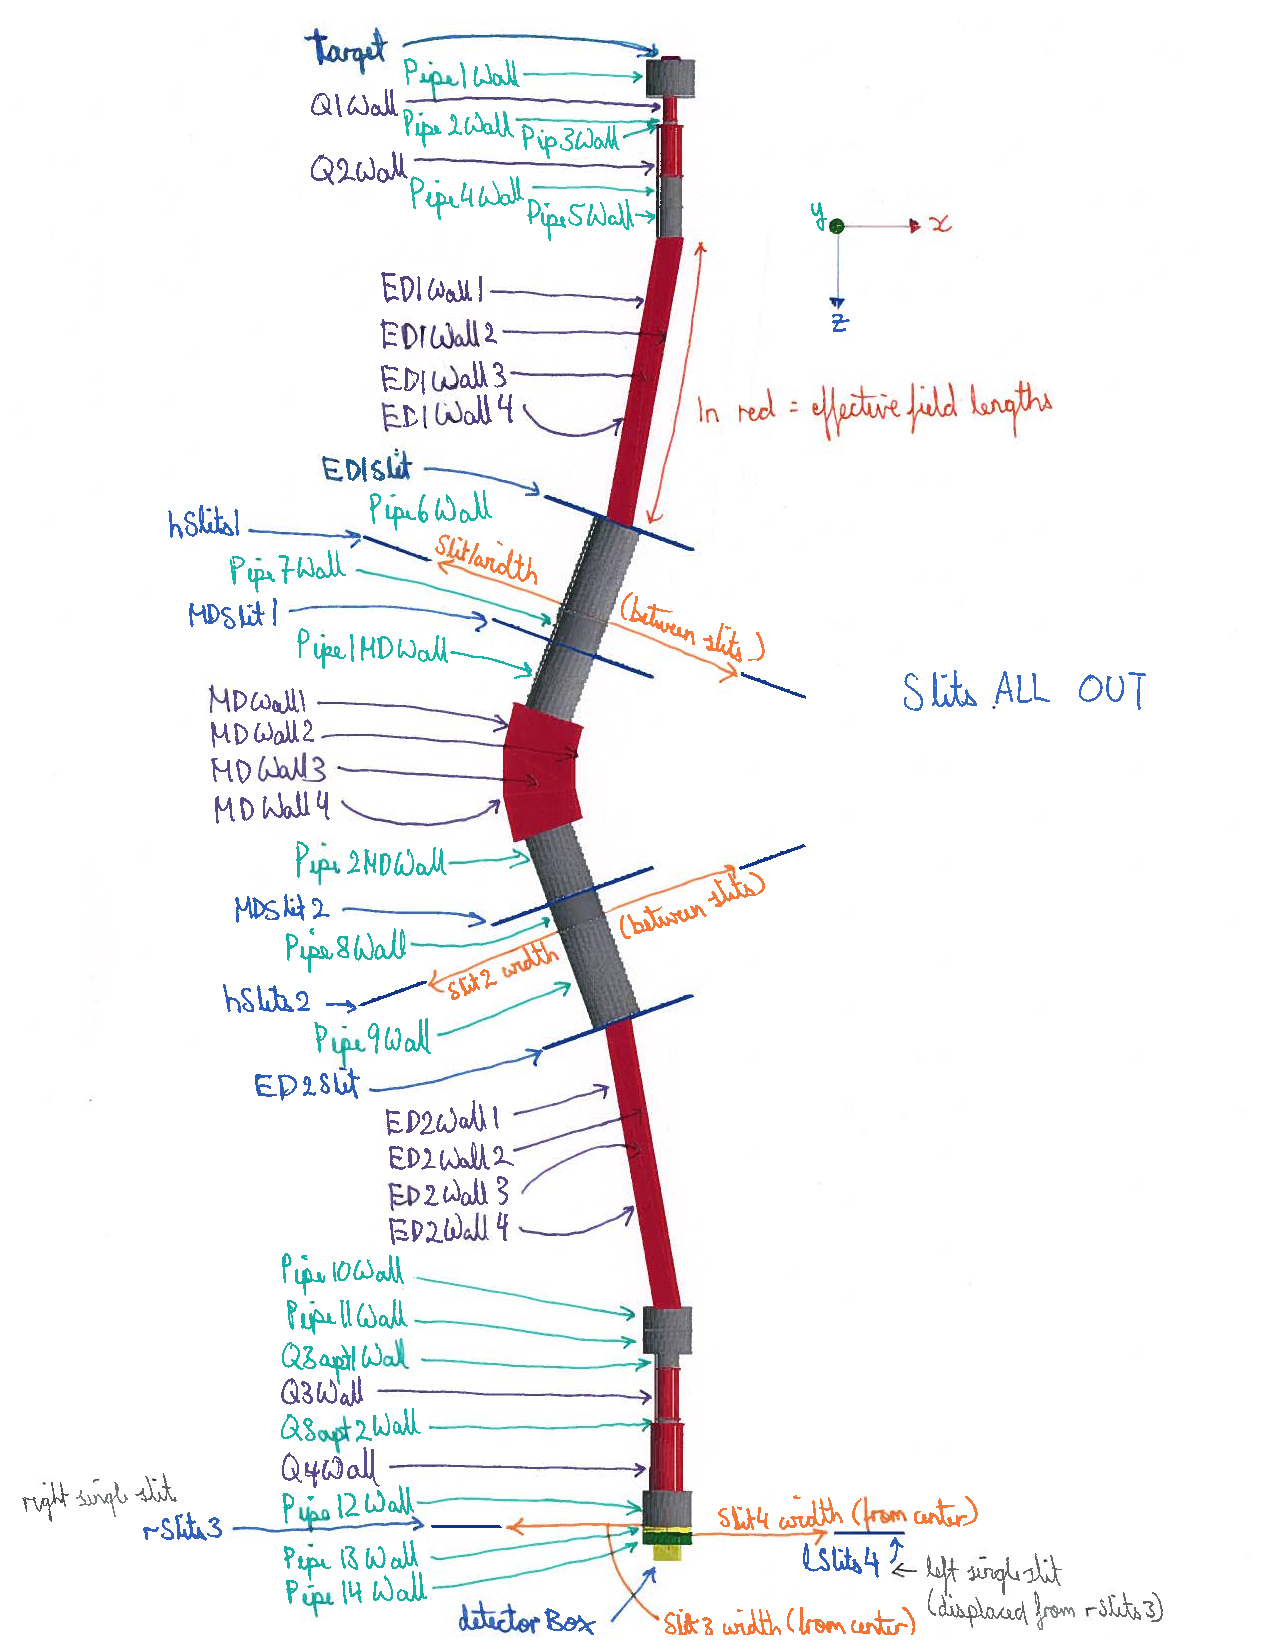
\includegraphics[width=0.9\textwidth]{graphs/EMMA_Wall_slitsOUT_labeled}
	}
	\caption{The EMMA target, slit, wall and detector volumes with all slits in the OUT position. This was plotted using viswalls.mac. Q, ED and MD stand for quadrupole magnet, electric dipole and magnetic dipole. The electric and magnetic field volumes are in order of Q1, Q2, ED1, MD, ED2, Q3 and Q4. The walls between ED1 and MD are at a 20$^{\circ}$ to the z-axis and -20$^{\circ}$ for the walls between ED2 and MD. The last two slits before the detector are single finger slits displaced in the z direction.}
	\label{fig:wallout}
\end{figure}

\begin{figure}
\centering
 	\subfloat{
      	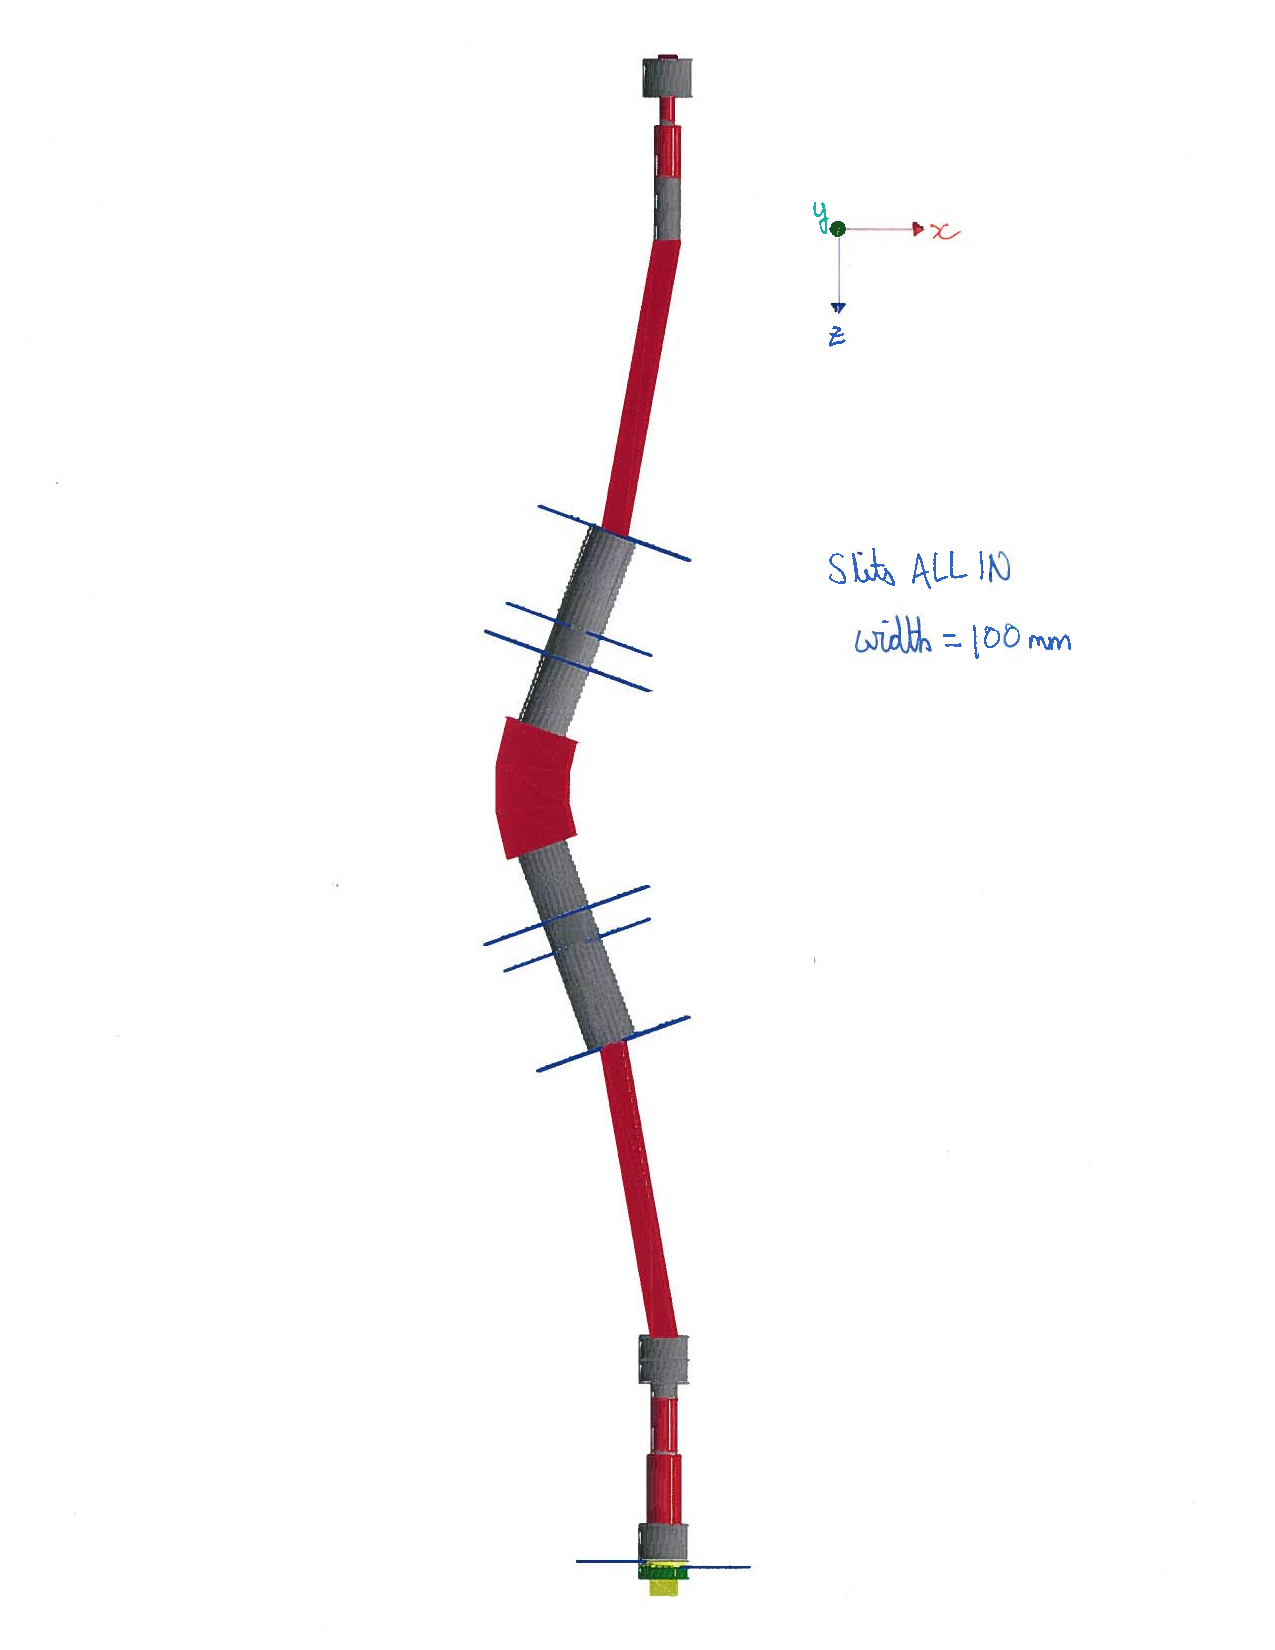
\includegraphics[width=0.9\textwidth]{graphs/EMMA_Wall_slitsIN_labeled}
	}
	\caption{The EMMA target, slit, wall and detector volumes with all slits 100 mm in. This was plotted using viswalls.mac.}
	\label{fig:wallin}
\end{figure}

The sizes of the volumes in SpectrometerConstruction.cc are determined by the effective field lengths and drift lengths listed in Table \ref{tab:lengths}. The effective field length is the path length where the particle 'feels' the electric or magnetic field. The drift lengths are the path lengths where the particle feels no field. If there are any discrepancies between this table and code, trust the code. I double and triple checked it. The walls and slits are all made out of aluminum and are arbitrarily 1 cm and 2 mm thick respectively.

\begin{table*}
\caption{Effective field lengths (EFL) and drift lengths (DL) given by Bruker}\label{tab:lengths}
\centering
\begin{threeparttable}
\begin{tabular}{ccc}
\hline
	&Length (cm)	&Logical volumes occupying length\\
\hline
DL	&22.75	&Pipe1WallLogical\\
EFL	&13.98	&Q1WallLogical\\
DL	&3.5		&Pipe2WallLogical\\
	&		&Pipe3WallLogical\\
EFL	&29.88	&Q2WallLogical\\
DL	&37.23	&Pipe4WallLogical\\
	&		&Pipe5WallLogical\\
EFL	&r=500, $\theta=20^{\circ}$\tnote{a}	&ED1Wall1Logical\\
	&		&ED1Wall2Logical\\
	&		&ED1Wall3Logical\\
	&		&ED1Wall4Logical\\
	&		&ED1SlitLogical\\
DL	&59.64	&Pipe6WallLogical\\
DL	&20.26	&hSlits1Logical\\
	&		&Pipe7WallLogical\\
	&		&MDSlit1Logical\\
DL	&42.6	&Pipe1MDWallLogical\\
EFL	&r=100, $\theta=40^{\circ}$\tnote{a}	&MDWall1Logical\\
	&		&MDWall2Logical\\
	&		&MDWall3Logical\\
	&		&MDWall4Logical\\
DL	&42.6	&Pipe2MDWallLogical\\
DL	&18.77	&MDSlit2Logical\\
	&		&Pipe8WallLogical\\
	&		&hSlits2Logical\\
DL	&61.13	&Pipe9WallLogical\\
EFL	&r=500, $\theta=20^{\circ}$\tnote{a}	&ED1SlitLogical\\
	&		&ED1Wall1Logical\\
	&		&ED1Wall2Logical\\
	&		&ED1Wall3Logical\\
	&		&ED1Wall4Logical\\
DL	&26.84	&Pipe10WallLogical\\
	&		&Pipe11WallLogical\\
DL	&9.65	&Q3apt1WallLogical\\
EFL	&29.88	&Q3WallLogical\\
DL	&3.0		&Q3apt2WallLogical\\
EFL	&40.18	&Q4WallLogical\\
DL	&20.92	&Pipe12WallLogical\\
DL	&3.2	&rSlits3Logical\\
	&		&Pipe13WallLogical\\
DL	&6.64	&lSlits4Logical\\
	&		&Pipe14WallLogical\\
\hline
\end{tabular}
     \begin{tablenotes}
       \item[a] {\small The EFL for the EDs and MD are curved and determined by the radius and bending angle.}
     \end{tablenotes}
\end{threeparttable}
\end{table*}

\newpage
\subsection{Vacuum regions and E and B fields}

Fig. \ref{fig:vac} shows the vacuum logical volumes.

\begin{figure}
\centering
 	\subfloat{
      	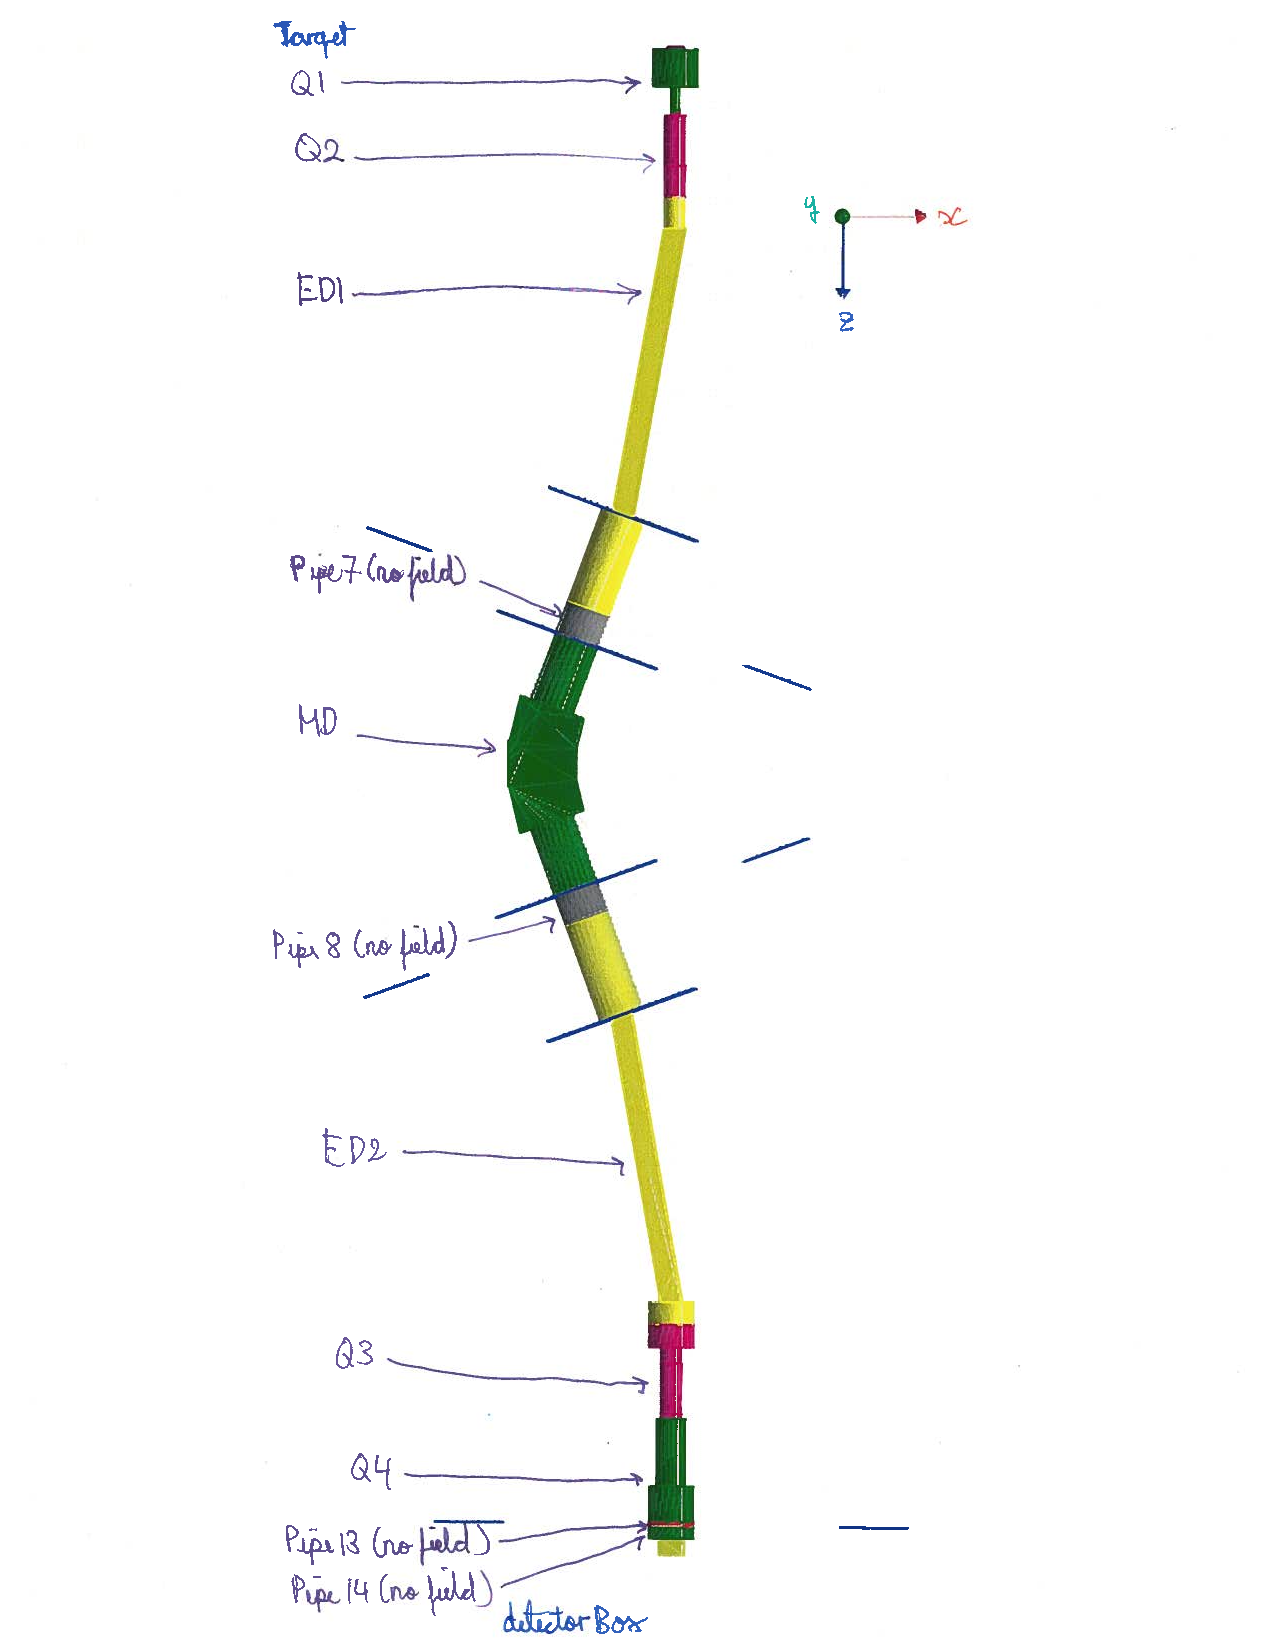
\includegraphics[width=0.9\textwidth]{graphs/EMMA_vacuum_labeled}
	}
	\caption{The EMMA vacuum volumes plotted using visvacuums.mac.}
	\label{fig:vac}
\end{figure}

The vacuum logical volumes are created in SpectrometerConstruction.cc and occupy the space inside the walls. The lengths are determined by the EFL and DL listed in Table \ref{tab:lengths}. The volumes with E and B fields are unions of several solids. The width and height or radius of the solids as well as the union of solids are listed in Table \ref{tab:vac}. All values unless indicated are give by Bruker. I made a comment where an arbitrary cylinder radius was used since I didn't know the dimensions, or for the case for Pipe1MDSolid and Pipe2MDSolid I didn't have time to implement the trapezoid shape show in Fig. \ref{fig:tetra}. This should be fixed later on but is a lower priority.

\begin{table*}
\caption{Vacuum logical volume properties}\label{tab:vac}
\centering
\begin{tabular}{ccccc}
\hline
Logical volume	&Field	&Union of solids &width x height or radius (cm)	& comments\\
\hline
Q1Logical	&BGField1.cc	&Pipe1Solid	&13.75	&arbitrary radius\\
		&			&Q1Solid		&3.1		&\\
		&			&Pipe2Solid	&3.1		&\\
Q2Logical	&BGField2.cc	&Pipe3Solid	&3.1		&\\
		&			&Q2Solid		&6.75	&\\
		&			&Pipe4Solid	&6.75	&\\
ED1Logical&BGField3.cc	&Pipe5Solid	&6.75	&\\
		&			&ED1Solid	&12.5 x 40	&\\
		&			&Pipe6Solid	&13.75	&arbitrary radius\\
Pipe7Logical	&		&Pipe7Solid	&13.75	&arbitrary radius\\
MDLogical&BGField4.cc	&Pipe1MDSolid	&13.75	&arbitrary radius\\
		&			&MDSolid		&40 x 12	&\\
		&			&Pipe2MDSolid	&13.75	&arbitrary radius\\
Pipe8Logical	&		&Pipe8Solid	&13.75	&arbitrary radius\\
ED2Logical&BGField5.cc	&Pipe9Solid	&13.75	&arbitrary radius\\
		&			&ED2Solid	&12.5 x 40	&\\
		&			&Pipe10Solid	&13.75	&arbitrary radius\\
Q3Logical	&BGField6.cc	&Pipe11Solid	&13.75	&arbitrary radius\\
		&			&Q3apt1Solid	&6.75	&\\
		&			&Q3Solid		&6.75	&\\
		&			&Q3apt2Solid	&6.75	&\\
Q4Logical	&BGField6.cc	&Q4Solid		&18.5	&\\
		&			&Pipe12Solid	&13.75	&arbitrary radius\\
Pipe13Logical	&		&Pipe13Solid	&13.75	&arbitrary radius\\
Pipe14Logical	&		&Pipe14Solid	&13.75	&arbitrary radius\\
\hline
\end{tabular}
\end{table*}

\begin{figure}
\centering
 	\subfloat{
      	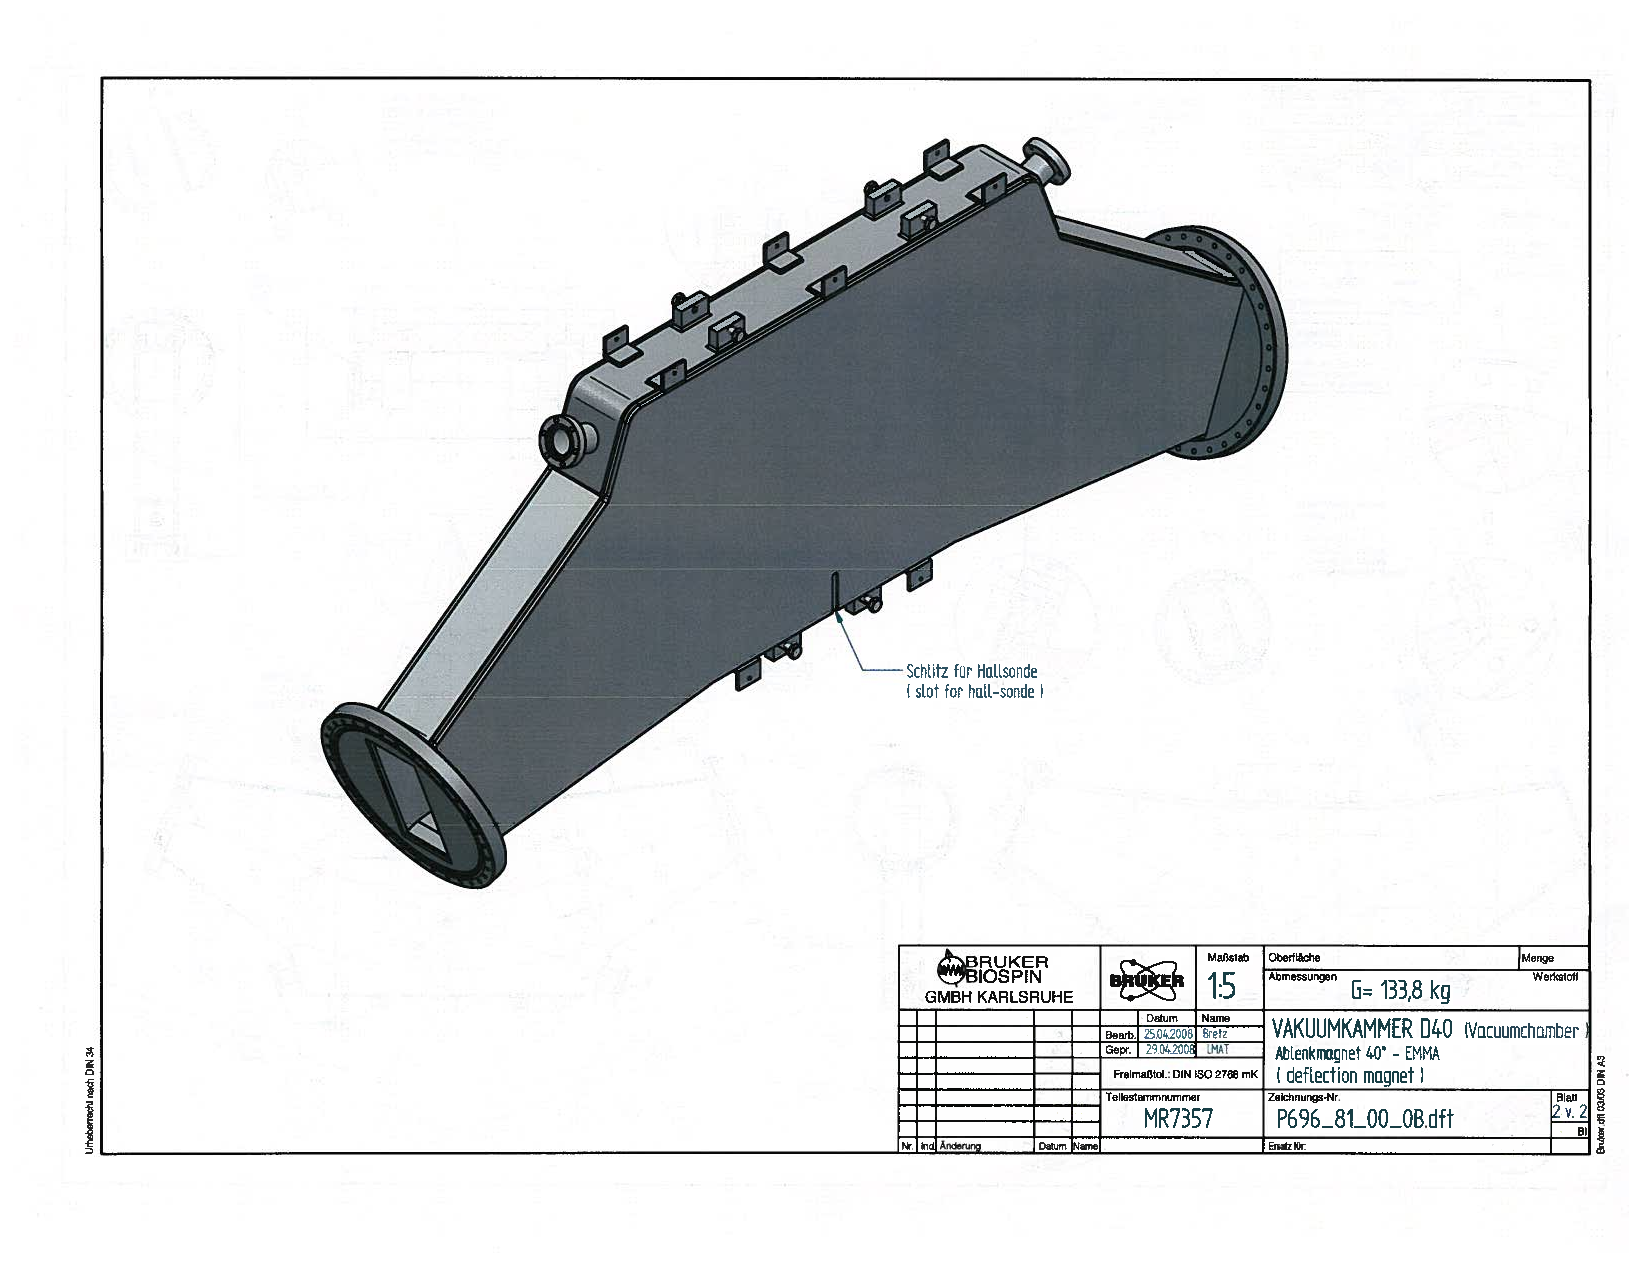
\includegraphics[width=0.8\textwidth]{graphs/MDvacuumbox}
	}\\
 	\subfloat{
      	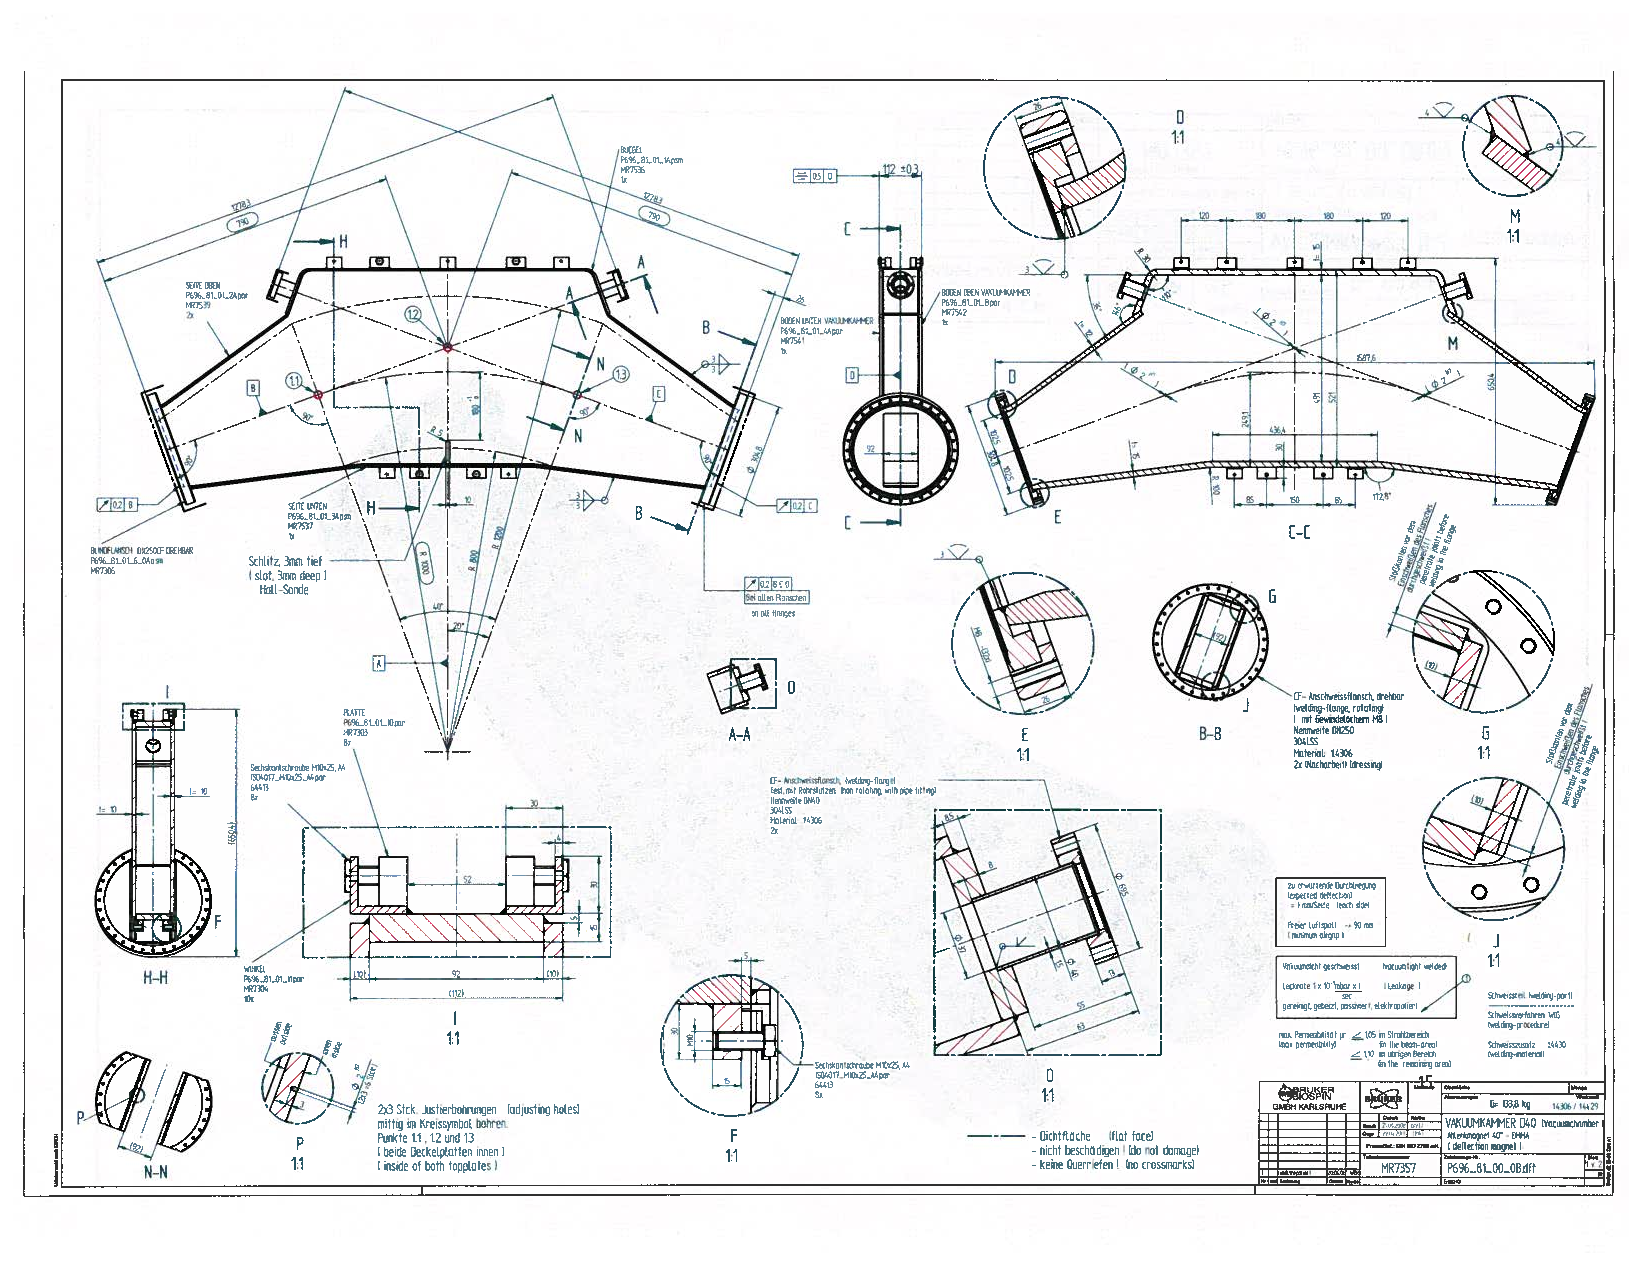
\includegraphics[width=0.8\textwidth]{graphs/MDvacuumboxspecs}
	}
	\caption{The MD drawings. Currently the effective field region (MDSolid) is described by a curved tube, which is correct, but the drift regions before and after the effective field region (Pipe1MDSolid and Pipe2MDSolid) are cylinders with an arbitrary radius of 13.75 cm. In the drawing the drift regions are trapezoids. You can get these drawings from Barry Davids.}
	\label{fig:tetra}
\end{figure}

\newpage
\subsection{Target and degraders}

The target and degraders are created in EMMADetectorConstruction.cc. Fig. {fig:degraders} shows the target, degrader and surrounding volumes if this target/degrader input file /UserDir/UserInput/targetDegraders.dat is used:
{\footnotesize \verbatiminput{inputfiles1.7/targetDegraders.dat}}
Extra volumes called Pipe0WallLogical and Pipe0Logical are created in between degrader 1 and 2, and Pipe1 is shortened. This is done so that there is no volume overlap between degrader 2 and Pipe1. The distance between the target and Q1 is still the same. In this file the target and degraders are 2 cm thick, REALLY thick. I did this so that you can see them when you plot the volumes, otherwise they would be too thin to see. They would be much thinner in reality. Currently the target and degraders are 10 x 10 cm in width and height. This can be changed.

\begin{figure}
\centering
 	\subfloat{
      	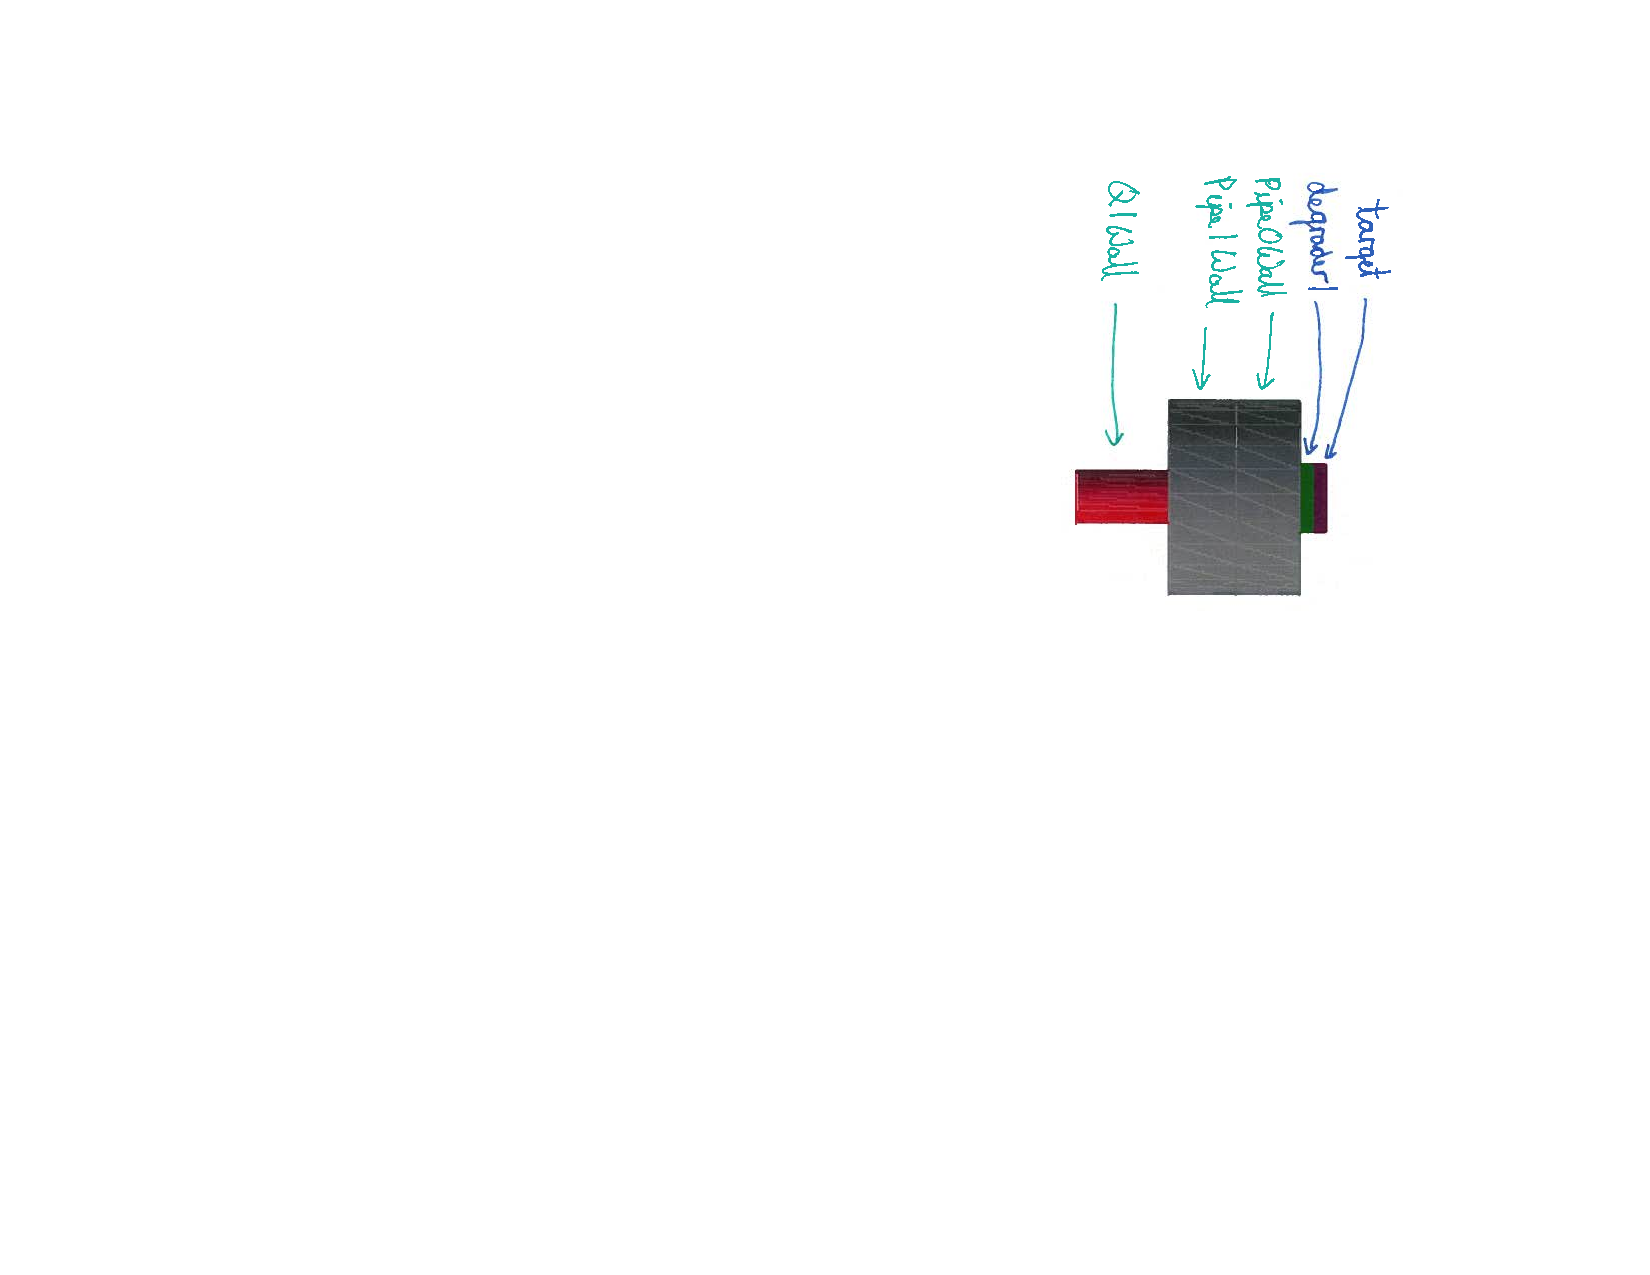
\includegraphics[width=0.5\textwidth]{graphs/EMMA_degraders1_labeled}
	}
 	\subfloat{
      	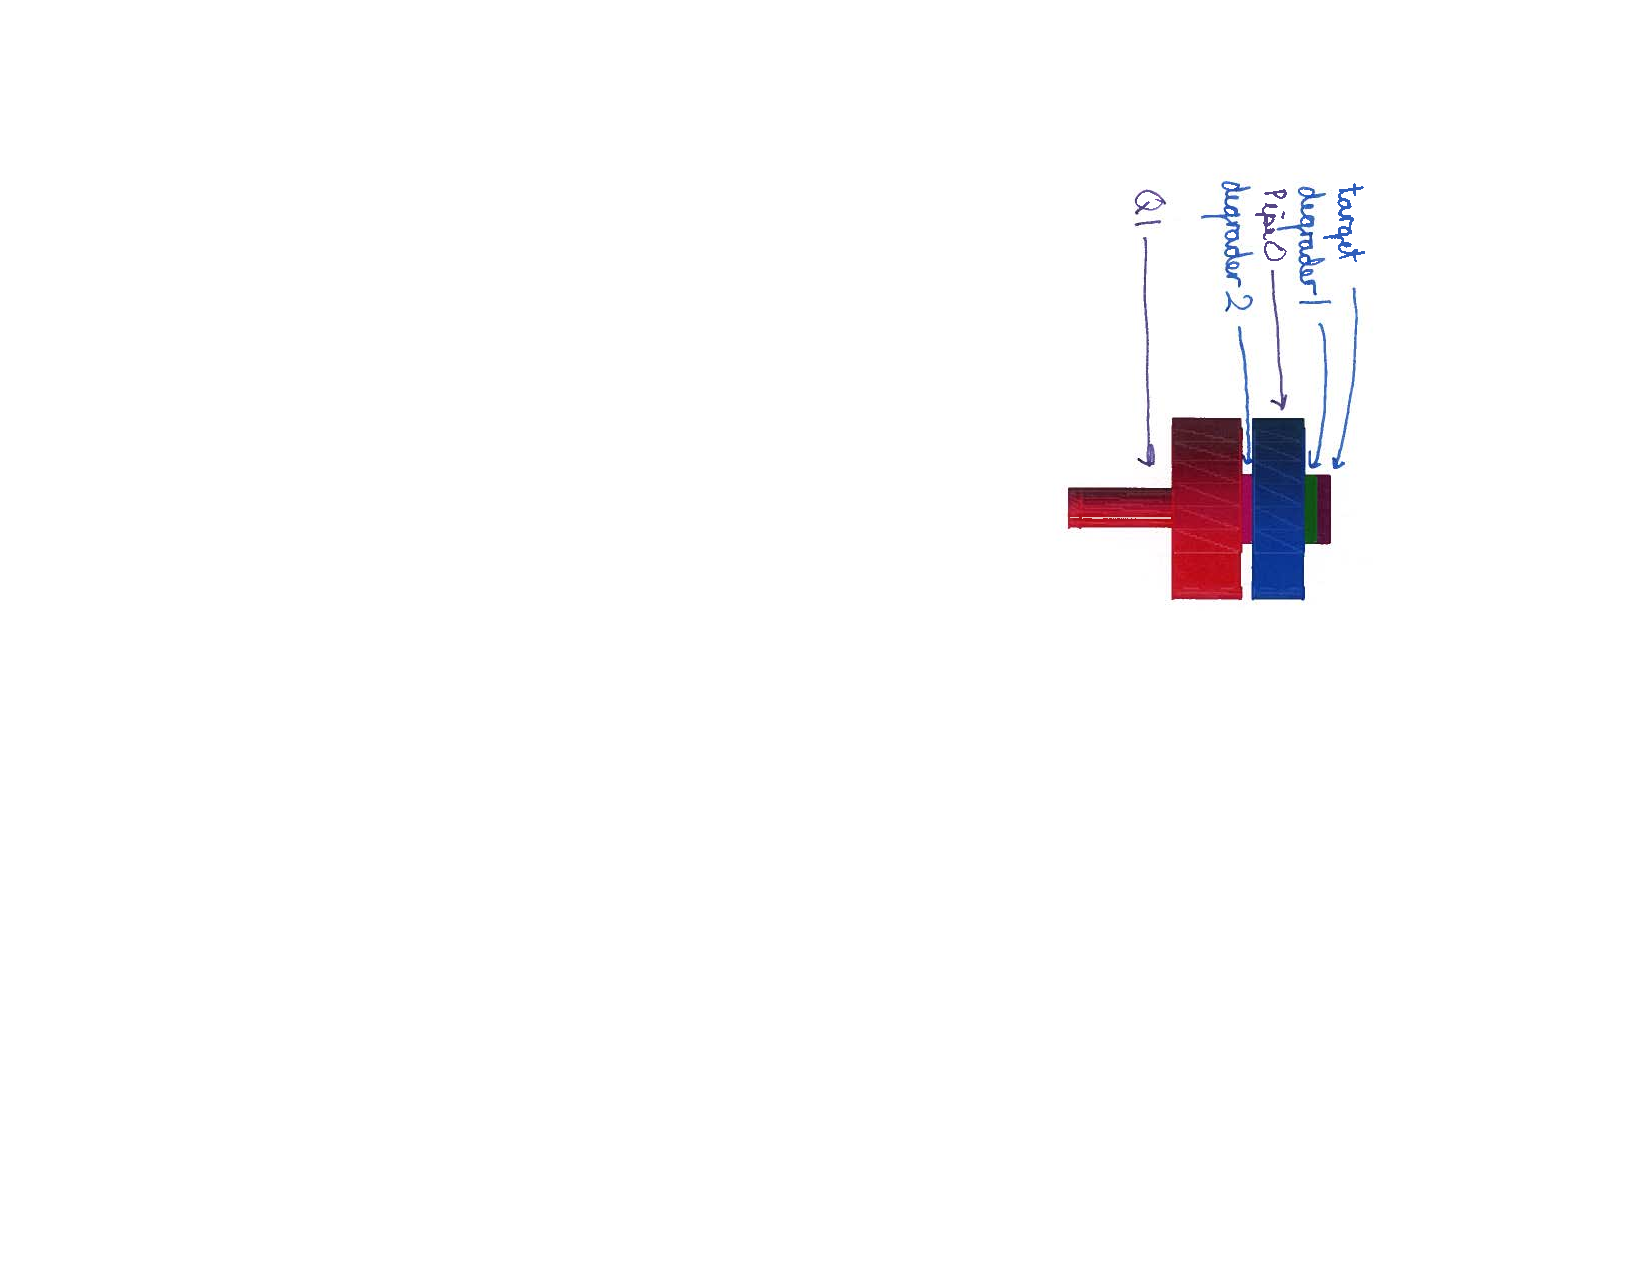
\includegraphics[width=0.5\textwidth]{graphs/EMMA_degraders2_labeled}
	}
	\caption{The target and degraders plotted using visdegraders.mac. On the left side I have plotted the walls and on the right the vacuum volumes underneath. You can see that Pipe0WallLogical covers the lengths of both Pipe0Logical and degrader2Logical.}
	\label{fig:degraders}
\end{figure}

\newpage
\subsection{Focal plane (detector) and PGAC (MWPC)}

EMMA uses a parallel grid avalanche counter (PGAC) to detect the particles a the end. PGAC is a multiwire proportional chamber (MWPC) containing isobutane gas. The focal plane is a set of vertical and horizontal wires inside the PGAC. The focal plane and the MWPC are created in EMMADetectorConstruction.cc. Currently the focal plane is a big box 15.4 x 5.4 cm and 20 cm thick made out of mylar. Fig. \ref{fig:detector} shows the current dimensions of the focal plane. The width of the focal plane and the dimensions and location of the MWPC are wrong and need to be fixed first. The detector and MWPC are created between lines 258 and 314 in EMMADetectorConstruction.cc. I haven't plotted the MWPC on any of the plots.

The PGAC spec drawing is shown in Fig. \ref{fig:pgac}a. It looks complicated but I figured the best way to represent it in Geant4 is by the drawing shown in Fig. \ref{fig:pgac}b. It should be an aluminum box with two windows made out of mylar, one at the entrance and one at the exit. You should find out from Franco Cifarelli, since he has all the drawings of the PGAC, what the window widths and heights are as well as the distance between the windows. The windows are 0.94 $\mu$m thick. The box is filled with isobutane gas. The pressure of the gas is a user input parameter specified in the /UserDir/UserInput/mwpc.dat file:
{\footnotesize \verbatiminput{inputfiles1.7/mwpc.dat}}
I think the MWPC should not be optional. Get rid of the first line. If the user defined pressure is zero put vacuum in the MWPC volume. The focal plane can be approximated by a thin mylar since you can't program the wires. The thickness should be chosen such that the particles lose little energy going through it but it should be larger than the Geant4 step length. If the focal plane is thinner than the step length some particles might step passed it and not get detected. Finally, find out the distance between the focal plane and one of the mylar windows to position it in the worldLogical volume. When you change the dimensions of the MWPC make sure you also change the length of Pipe14WallLogical and Pipe14Logical in SpectrometerConstruction.cc to avoid volume overlaps.

\begin{figure}
\centering
 	\subfloat{
      	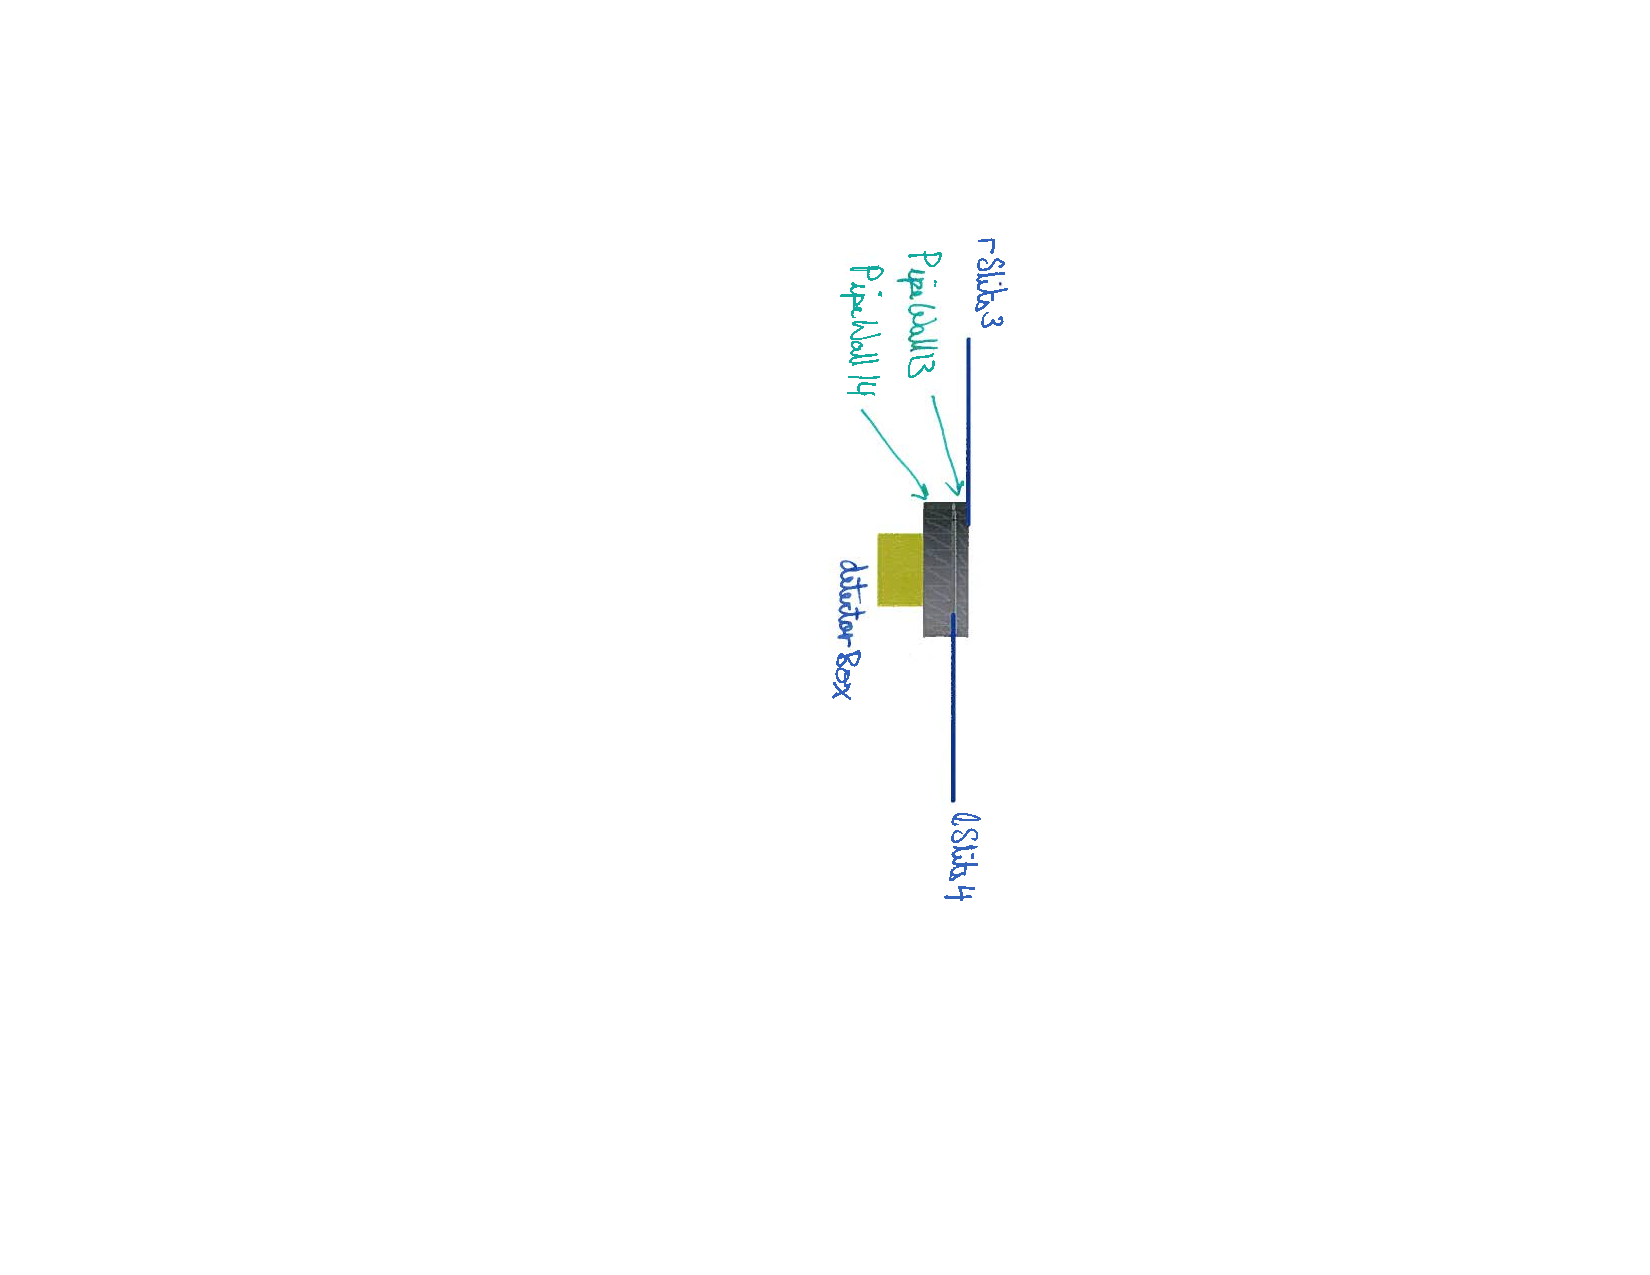
\includegraphics[width=0.15\textwidth]{graphs/EMMA_detector_labeled}
	}
	\caption{The current focal plane (detectorBox) of EMMA plotted using visdetector.mac. The front of the focal plane is at the correct location but it's too wide.}
	\label{fig:detector}
\end{figure}

\begin{figure}
\centering
 	\subfloat[]{
      	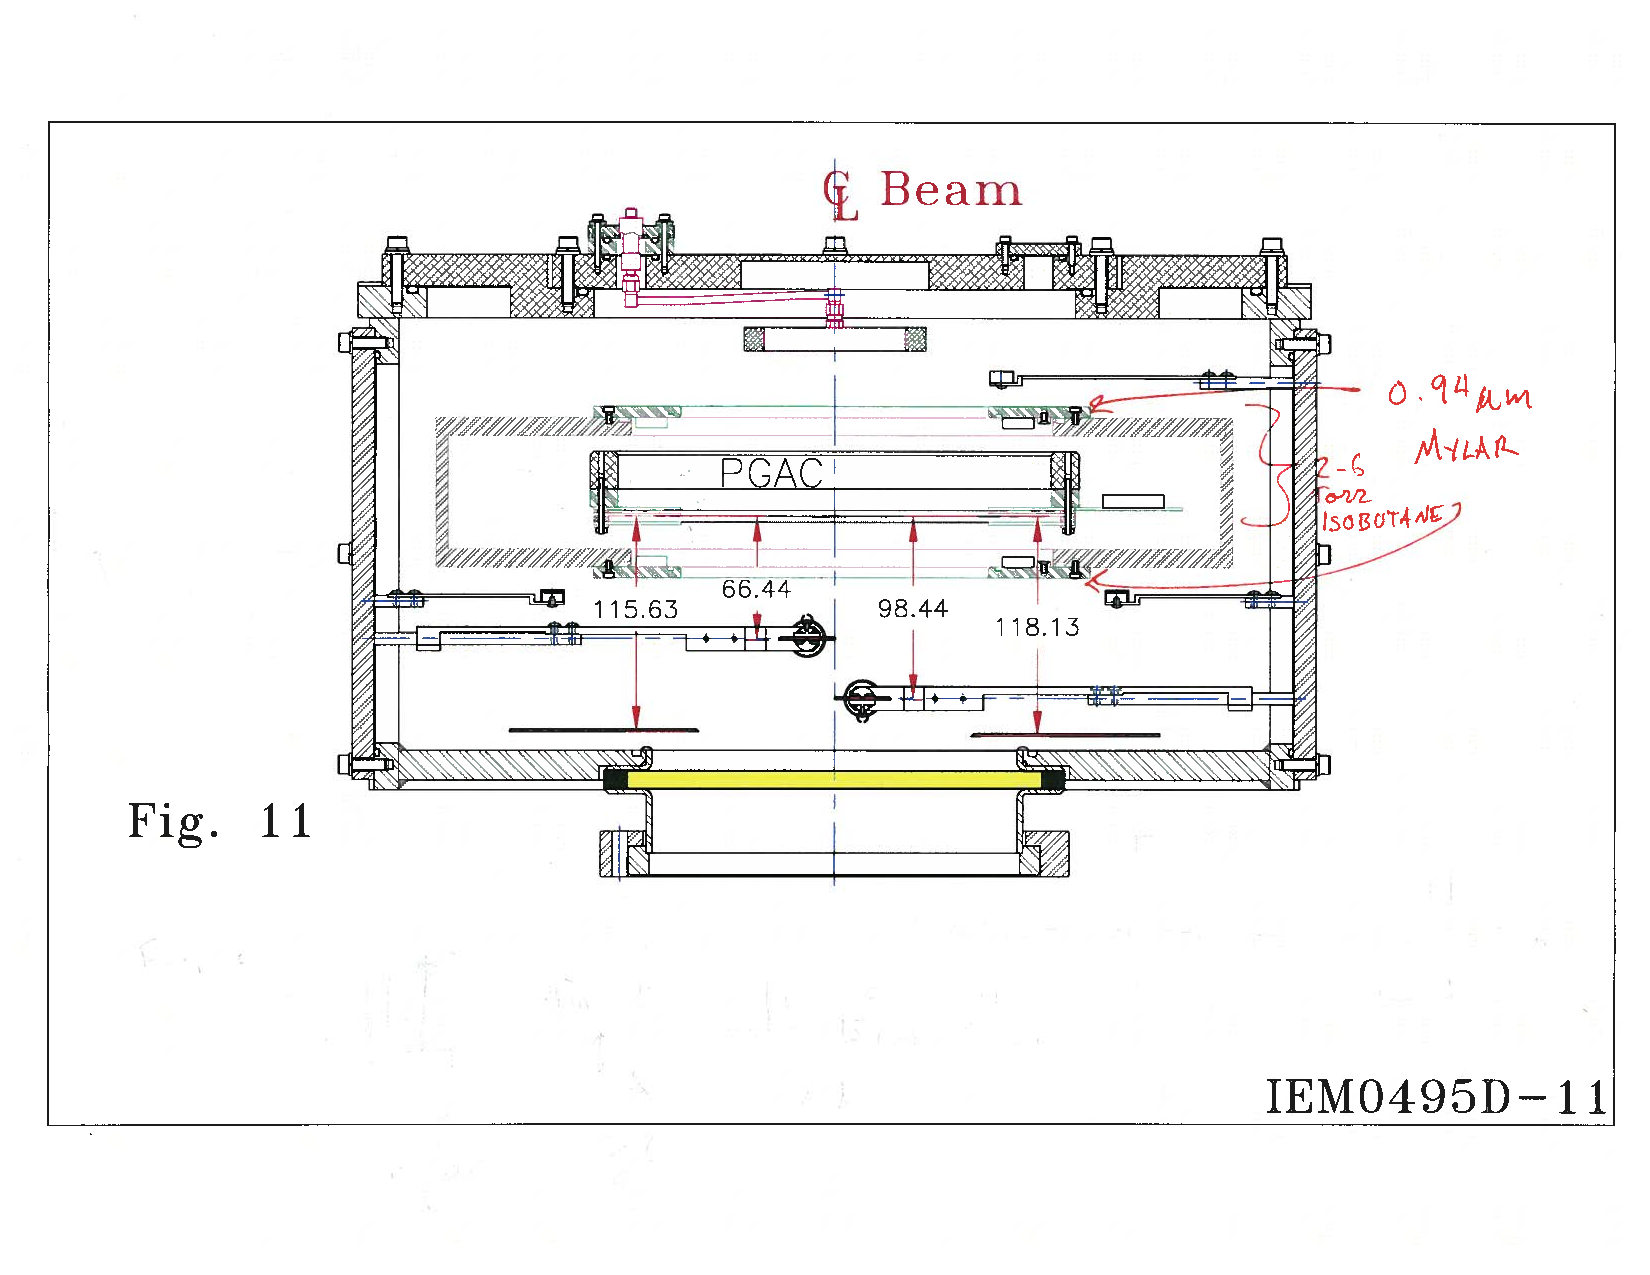
\includegraphics[width=0.9\textwidth]{graphs/PGACspecs}
	}\\
 	\subfloat[]{
      	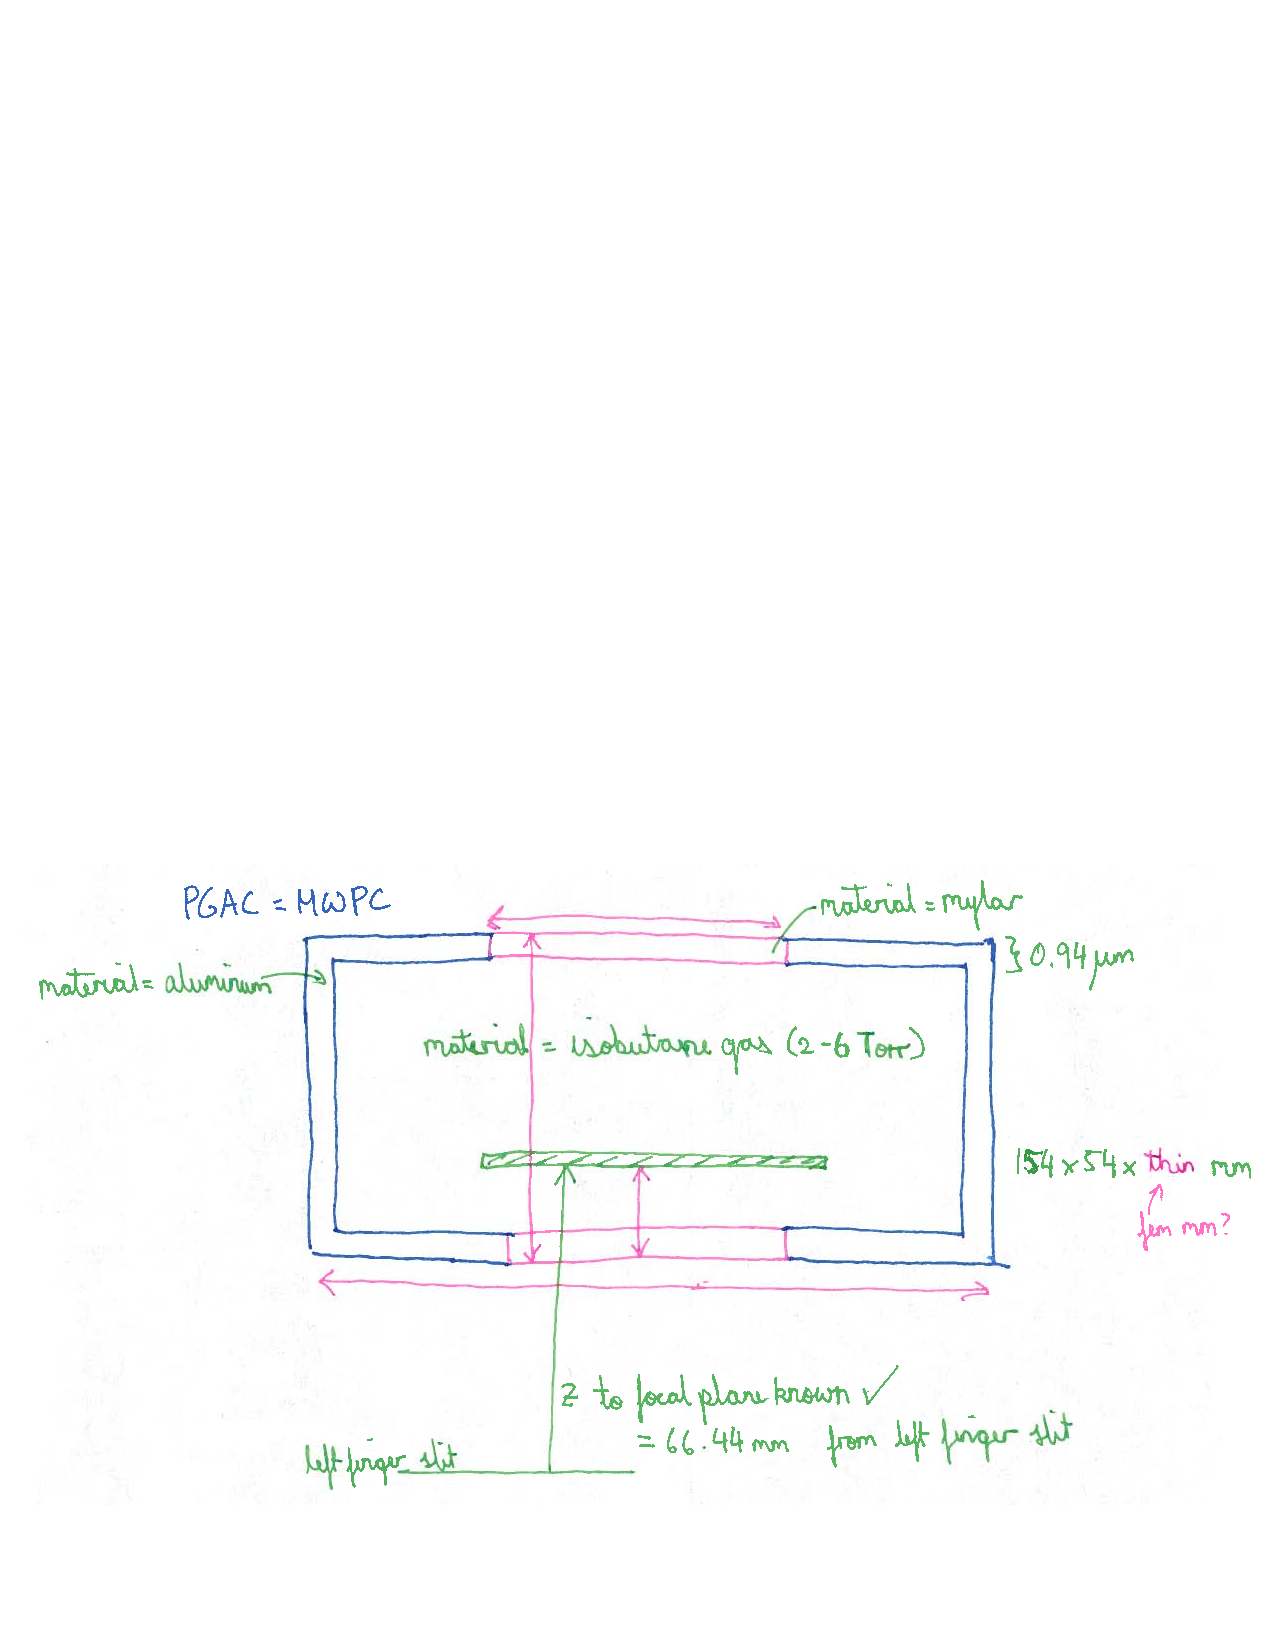
\includegraphics[width=0.7\textwidth]{graphs/PGACgemma}
	}
	\caption{The PGAC drawing and my version of how I think it should be implemented in the Geant4 code. See text for detailed description.}
	\label{fig:pgac}
\end{figure}

\subsection{To do list}

\textcolor{red}{To do list for the BGField classes:
\begin{enumerate}
\item Correct how the MWPC and focal plane are implemented in EMMADetectorConstruction.cc (lines 258 to 314). Use Fig. \ref{fig:pgac}b as a guide of how the MWPC should look in the simulation. First find out the height and width of the mylar windows, the distance between the focal plane and one of the windows, the distance between the two windows and choose a thickness for the focal plane. Then you'll have all the necessary dimensions and positions to add the MWPC.
\item Low priority: Implement the correct shapes for volumes commented with an ``arbitrary radius'' in Table \ref{tab:vac}. An example shown in Fig. \ref{fig:tetra} where Pipe1MDSolid and Pipe2MDSolid are not cylinders but actually trapezoids. Ask Barry Davids for drawings of these parts.
\end{enumerate}
}


\newpage
\section{Electric (E) and Magnetic (B) Field Implementations}

\subsection{BGField classes}

The E and B field calculations are done with the BGField classes:

\begin{enumerate}
\item BGField1.cc for Q1 (quadrupole magnet)
\item BGField2.cc for Q2
\item BGField3.cc for ED1 (electric dipole)
\item BGField4.cc for MD (magnetic dipole)
\item BGField5.cc for ED2
\item BGField6.cc for Q3
\item BGField7.cc for Q4
\end{enumerate}
Note: sometimes I will write BGFieldn.cc, where n=1 to 7, to talk about all 7 field classes at once.

The fields are added to the union solid logical volumes in SpectrometerConstruction.cc as listed in Table \ref{tab:vac}. Here is an example of how the B field is added to Q1 (lines 215 to 221). This is done similarly for the other electromagnetic elements:

\filefont{
    Field1 = new BGField1(0,zQ1fieldbegins,Pipe1HL*2,Pipe2HL*2); //see BGField1.cc for description of input parameters\\
    G4int nvar = 8; //nav set for all B and E fields\\
	G4EqMagElectricField* MagEquation1 = new G4EqMagElectricField(Field1);\\
	G4MagIntegratorStepper* MagStepper1 = new G4ClassicalRK4(MagEquation1,nvar);\\
	G4ChordFinder* MagChordFinder1 = new G4ChordFinder(Field1,minStep,MagStepper1);\\
	G4FieldManager* fieldMgr1 = new G4FieldManager(Field1,MagChordFinder1);\\
	G4LogicalVolume* Q1Logical = new G4LogicalVolume(Q1Union,Vacuum,"Q1Logical", fieldMgr1,0,0);\\
}

You create the field using\\
\filefont{Field1 = new BGField1(0,zQ1fieldbegins,Pipe1HL*2,Pipe2HL*2);}\\
The first two input parameters of the BGField classes are the x and z positions of where the volume begins. Everything is centered around y=0, so we can omit anything to do with y-offsets. The third input parameter is the distance along the optical axis (not the world logical volume axis) between the front of this volume and the edge of the effective field. The optical axis follows the central path through all volumes. The fourth input parameter is the distance along the optical axis between the edge of the effective field and the end of the volume. I don't understand the lines in between, but I know that the field is them added to the logical volume called \filefont{Q1logical} in the last line:\\
\filefont{G4LogicalVolume* Q1Logical = new G4LogicalVolume(Q1Union,Vacuum,"Q1Logical", fieldMgr1,0,0);}

If you look at what the \filefont{BGField1} object does in BGField1.cc you can see that there are a lot more parameters, in the  \filefont{data} array. These are the hardcoded input parameters needed to calculate the B field in Q1. I have labeled the effective field length and the poll radius, but I didn't have time to figure out what all the other uncommented parameters mean. The \filefont{GetFieldValue(const double Point[3],G4double $^{*}$Bfield)} object is called by geant when a particle passes through the \filefont{Q1Logical} volume. At each step \filefont{Point[3]}, the location in the world logical volume, is passed through to the object and the \filefont{Bfield} is calculated.

The \filefont{mitray\_poles\_\_(data,pos,field);} function does the field strength calculations from the \filefont{data} parameters and at the \filefont{pos}, the location wrt to the \filefont{Q1Logical} volume. \filefont{pos} is calculated from \filefont{Point[3]} and the x and z position of where the \filefont{Q1Logical} volume begins. For the EDs \filefont{mitray\_edipol\_\_} and for the MD \filefont{mitray\_dipole\_\_} are called. These functions are taken from \filefont{ray.f}, a fortran program written by Prof. Stanley Kowalski at MIT and calculates field strengths for different types of magnetic and electric fields. \filefont{ray.f} is found in the RAYTRACER zip file in the /fortran/ folder. Derek Howell (I believe) extracted the relevant subroutines for the electric dipoles, magnetic dipoles and quadrupoles, and created files called mitray\_dipol.f etc, in the /fortran/ folder. These were then converted from fortran to c and a c++ file called /fortran/mytray.cc was created. This later file is used in gemma1.7. I didn't look into this nor check if it was done correctly, so this needs to be done.
 
I will add a few more things that I have figured out about the BGField classes. The \filefont{mitray} functions use the position relative to the electromagnetic volume \filefont{pos} and not the \filefont{worldLogical} volume \filefont{Point}. All lengths and distances must be specified in cm.

The effective field length (EFL) is the length of the field along the optical axis in which the particle feels the field. For each quad the EFL is specified in \filefont{data[11]} and the optical axis is a straight line along the z-axis. The EDs and MD, and hence the optical axes, are bent so the EFLs are calculated using the radius of the curvature, $r=$\filefont{data[13]}, and the subtended angle, $\theta_{sub}=$\filefont{data[15]}:
\begin{equation}\label{eq:eflcurve}
EFL=\frac{\theta_{sub}}{360}2\pi r
\end{equation}
There is a bug in how the fields are calculated and the output EFL is not the same as the specified input EFL. So, as a temporary fix the input EFL of the EDs and MD can be modified such that we get the desired output EFL. Without the modified input there is a 0.1\% difference in the input and output EFL for the EDs and 0.25\% difference for the MD. This results in a $\sim$10 mm difference at the focal plane. The input EFLs hasn't been modified for the quads yet, however a small difference in the EFL for the quads isn't that critical. Having the correct EFL for ED1, MD and ED2 is far more critical! Table \ref{tab:efl} shows the input parameters I used. I describe in Section \ref{sec:efl} and \ref{sec:eflcalc} how I calculated the output EFLs.

\begin{table*}
\caption{Effective field length (EFL) inputs \filefont{data[11]}, \filefont{data[13]} and \filefont{data[15]}}\label{tab:efl}
\centering
\begin{tabular}{ccccc}
\hline
	&EFL (cm)	&Radius (cm)	&Angle specification (deg)	&Angle modified(deg)\\
\hline
Q1	&13.977		&&&\\
Q2	&29.88		&&&\\
ED1	&			&500			&20			&20.002605\\
MD	&			&100			&40			&39.89865\\
ED2	&			&500			&20			&20.02425\\
Q3	&29.88		&&&\\
Q4	&40.18		&&&\\
\end{tabular}
\end{table*}

For the quads the poll radius \filefont{data[12]} is the distance between the center and the poll tips of the magnets. The particles are travelling through a cylindrical vacuum chamber in between the magnets with a smaller aperture than the poll radius. To define the volume of the quads in SpectrometerConstruction.cc the aperture of the vacuum chamber is used. The poll radius $r=$\filefont{data[12]} is used to define the magnetic fields in the, e.g. BGField1.cc. Table \ref{tab:poll} lists the poll radius and the vacuum chamber aperture of the quads given by Bruker's specification.

\begin{table*}
\caption{Radii of the poll tips and vacuum tube aperture of quads}\label{tab:poll}
\centering
\begin{tabular}{ccc}
\hline
	&Poll tip radius (cm)	&Vacuum chamber aperture radius (cm)\\\\
\hline
Q1	&3.5		&3.1\\
Q2	&7.5		&6.75\\
Q3	&7.5		&6.75\\
Q4	&10		&9.25\\
\end{tabular}
\end{table*}

The initial field strengths \filefont{FieldStrength\_0} are calculated or measured from a $Z=54$ particle with mass $A=500$ AMU, charge $Q=20$ and energy $E=180$ MeV. All reference \filefont{FieldStrength\_0} values used are listed in Table \ref{tab:fields}. The field strengths for the quads were given by Bruker. Those of the ED1, ED2 and MD are calculated from the electric and magnetic rigidities. The rigidities are given in line 516 and 517 of EMMADetectorConstruction.cc\\
\filefont{  // reference rigidities\\
  G4double magneticRigidity\_0 = 289.672643165132; // Z=54, A=100, Q=20, E=180 MeV\\
  G4double electricRigidity\_0 = 17.9826410468929; // Z=54, A=100, Q=20, E=180 MeV}\\
and are calculated using equations
\begin{align}
B_{rigidity}=mv/q\\
E_{rigidity}=mv^{2}/q
\end{align}
For the MD \filefont{FieldStrength\_0} in BGField4.cc is simply the magnetic rigidity (line 516) multiplied by \filefont{1./(2.99792458e2)} to convert it to units of T m. For the ED \filefont{FieldStrength\_0} in BGField3.cc and BGField5.cc is twice the electric rigidity (line 517) in units of kV/cm. The fields are then scaled using the $Z$, $A$, $Q$ and $E$ of the particle we specify in the /UserDir/UserInput/centralTrajectory.dat file. The scaling factors are calculated in the CalculateScalingFactors() object of EMMADetectorConstruction.cc (line 513 onwards) and \filefont{FieldStrength\_0}, in the BGFieldn.cc, are scaled in using (line 568)\\
\filefont{Spectrometer->ScaleFieldStrength( magneticScaling, electricScaling )}.\\
\filefont{Spectrometer} is a \filefont{SpectrometerConstruction} type and is defined in line 249 of EMMADetectorConstruction.cc.

\begin{table*}
\caption{Field strengths of the reference particle}\label{tab:fields}
\centering
\begin{tabular}{ccc}
\hline
	&B (Tm)	&E (kV/cm)\\\\
\hline
Q1	&1.37991		&\\
Q2	&-0.89239		&\\
ED1	&			&-35.9653\\
MD	&0.96624		&\\
ED2	&			&-35.9653\\
Q3	&-0.60653		&\\
Q4	&0.77907		&\\
\end{tabular}
\end{table*}

After the B fields are calculated, using the \filefont{mytray} functions in the \filefont{GetFieldValue(const double Point[3],G4double $^{*}$Bfield)} objects, they are scaled by the charges \filefont{userCharge/currentCharge}.\\\filefont{G4double userCharge = 54.; // default value}\\
is the reference particle $Z$ value defined first as a global variable in line 69 of EMMAPrimaryGeneratorAction.cc. This value is then changed in the \filefont{GeneratePrimaries(G4Event* anEvent)} object in the same class, to set it to the $Z$ value of the particle you are simulating.\\
\filefont{G4double currentCharge = 0.0; // default value is 0}\\
is defined in line 51 of EMMASteppingAction.cc. It is changed in line 122 in the \filefont{UserSteppingAction(const G4Step$^{*}$ theStep)} object of EMMASteppingAction.cc:\\
\filefont{currentCharge = theCharge}\\
which is not equal to zero. I'm not sure what the \filefont{currentCharge} parameter exactly is so I don't understand this charge scaling factor.

Another issue with how the B fields are implemented in the quads is that due to the proximity the fields between Q1 \& Q2 and Q3 \& Q4 overlap. These interference are not taken into account. Currently there is a sharp boundary between the quads and the field is cutoff at the boundary. Fig. \ref{fig:quads} shows this. This is unphysical and needs to be changed. Due to the changes in the lengths of the drift spaces and the addition of slits the entrance field of ED1 and exit field of ED2 are also cutoff. This can be seen in Fig. \ref{fig:dipoles}. In fact there will be an E field overlap in the Q2 volume from ED1 and the same for ED2 and Q3. This must be accounted for as well.

\begin{figure}
\centering
 	\subfloat{
      	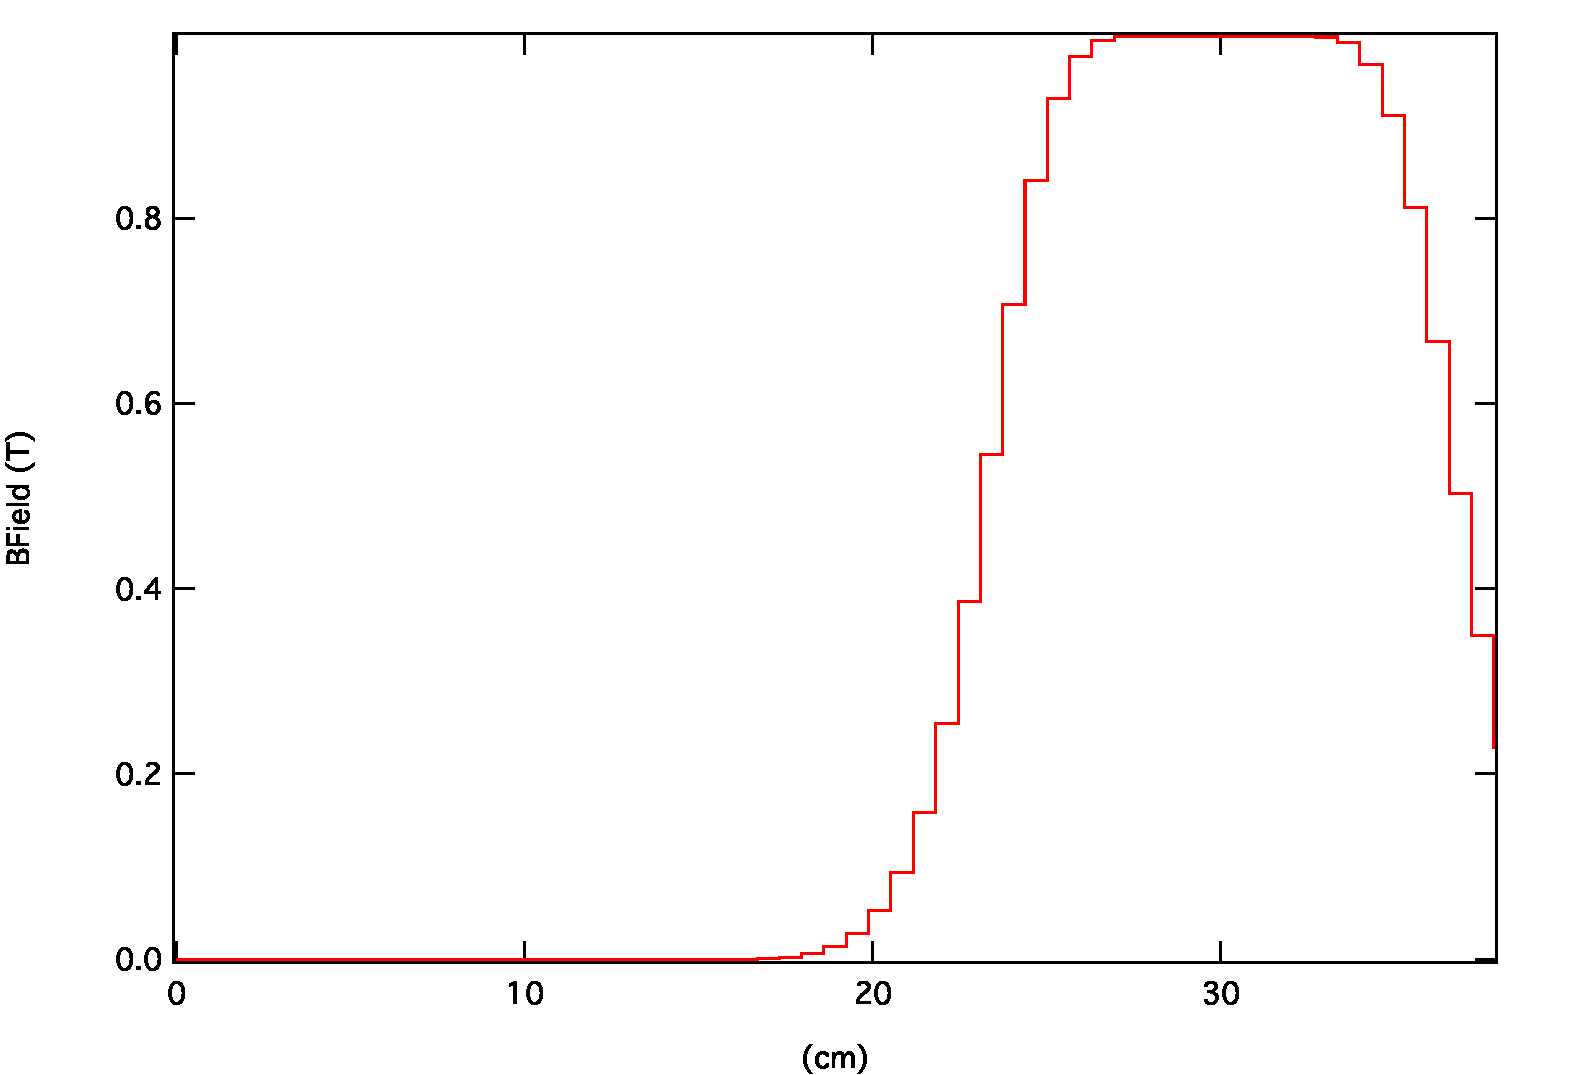
\includegraphics[width=0.5\textwidth]{graphs/Q1cutoff}
	}
	\subfloat{
	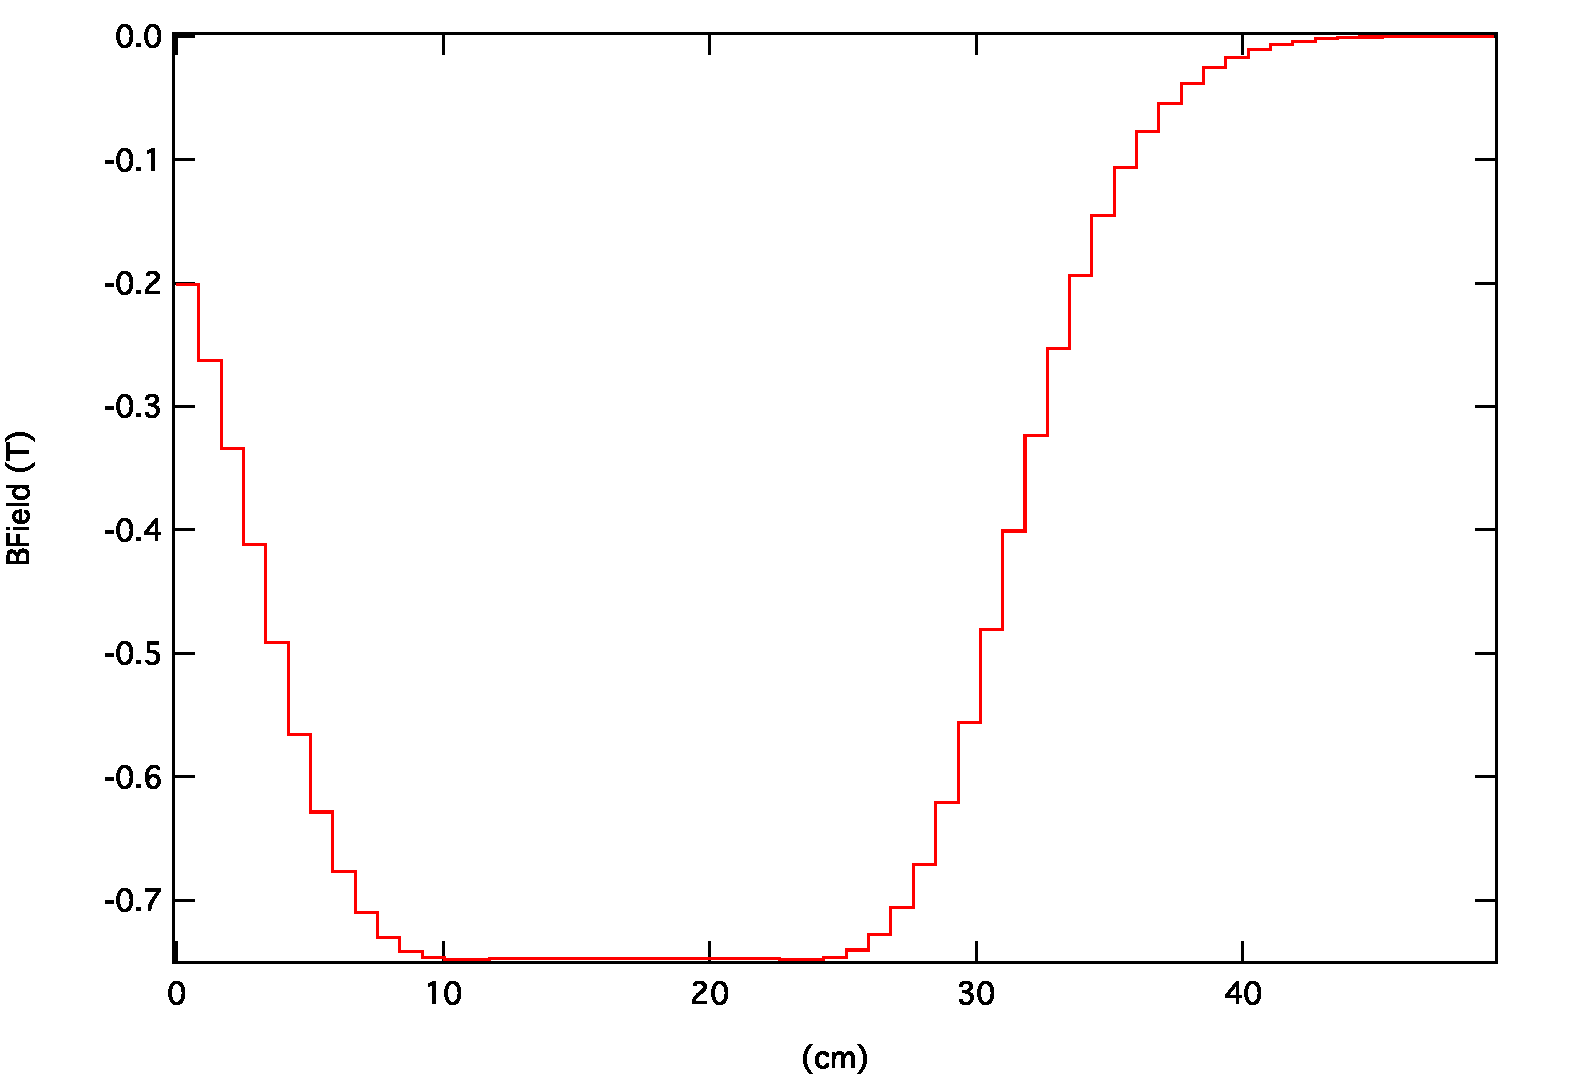
\includegraphics[width=0.5\textwidth]{graphs/Q2cutoff}
	}\\
 	\subfloat{
      	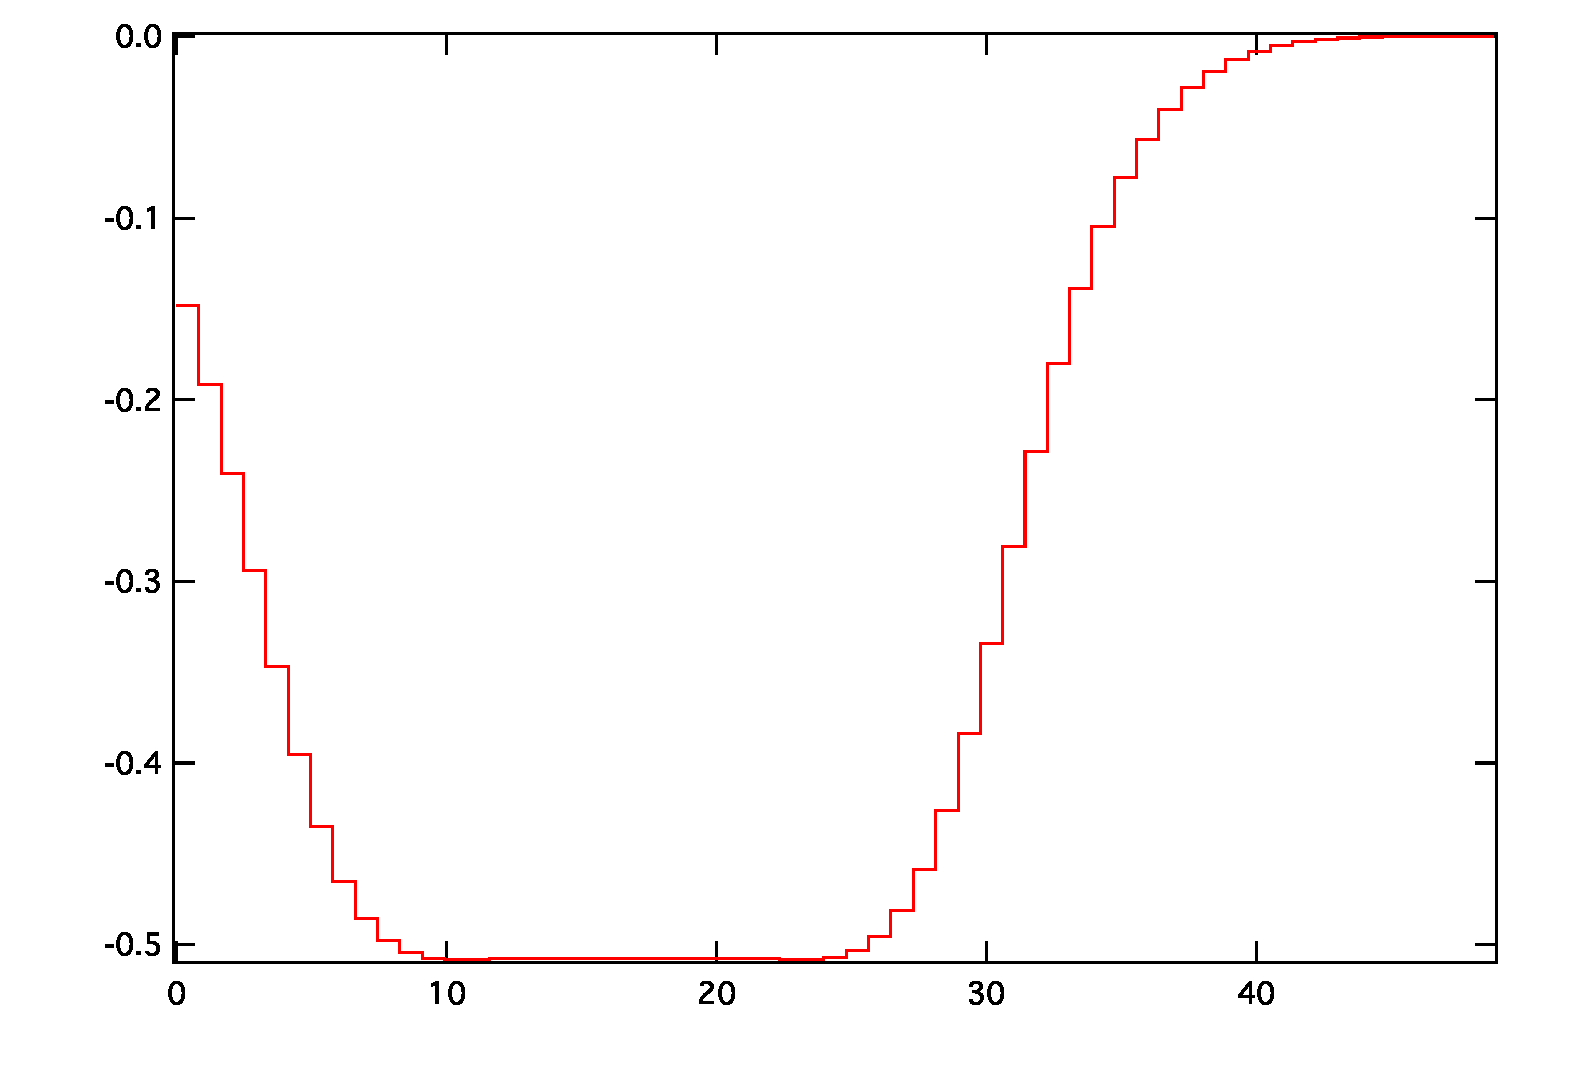
\includegraphics[width=0.5\textwidth]{graphs/Q3cutoff}
	}
	\subfloat{
	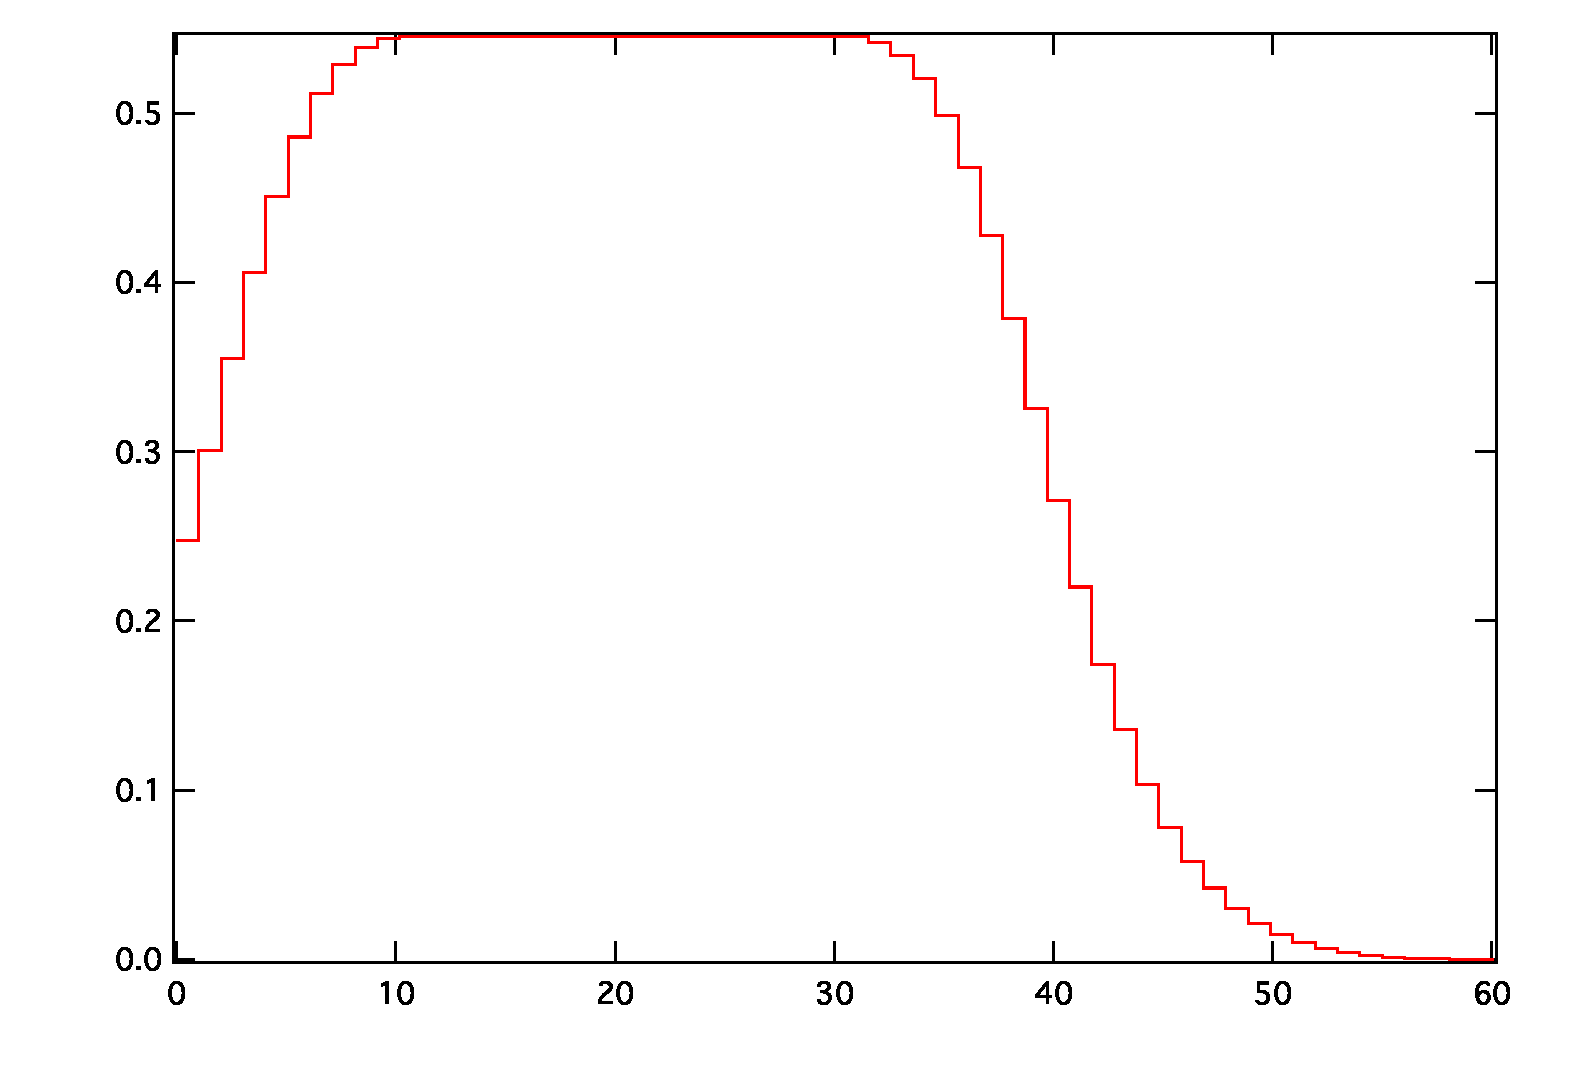
\includegraphics[width=0.5\textwidth]{graphs/Q4cutoff}
	}
	\caption{The change in B field through Q1, Q2, Q3 and Q4. Since the fields currently have a sharp boundary they are cutoff at the boundary. When eventually the correct magnetic field interferences are added the field going from the top left graph (Q1) to the top right graph (Q2) should be a continuous transition since they are right next to each other, and the same should be true for the bottom two graphs for Q3 and Q4.}
	\label{fig:quads}
\end{figure}

\begin{figure}
\centering
 	\subfloat{
      	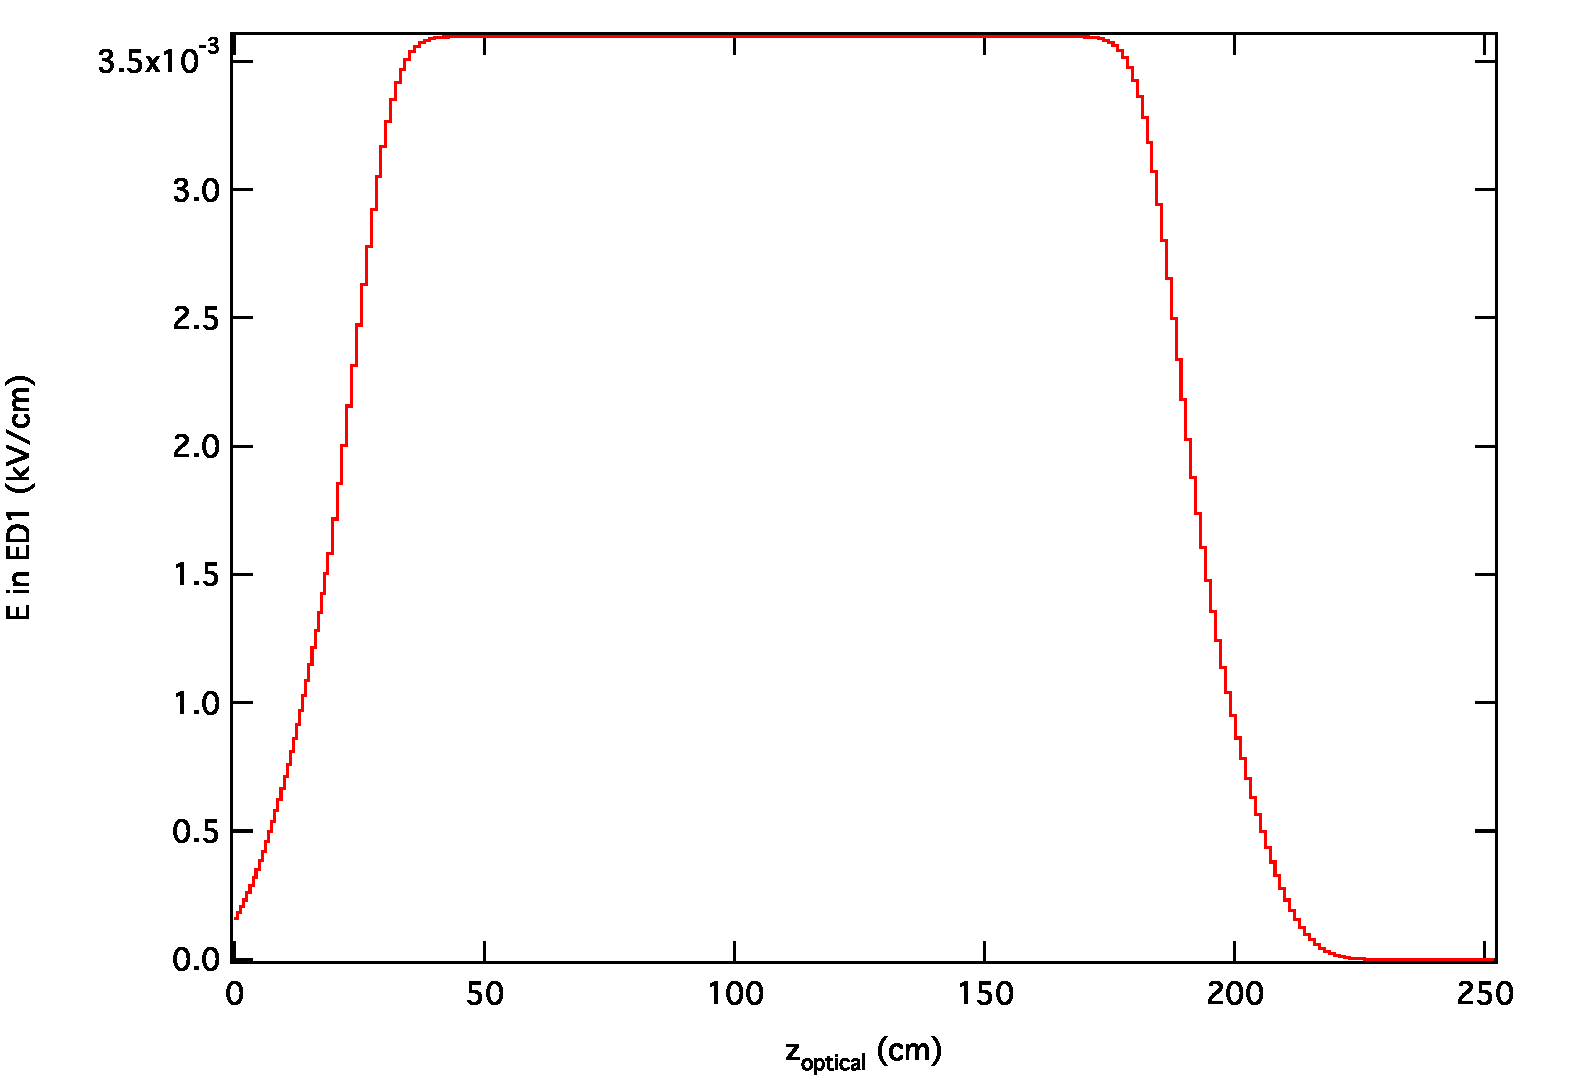
\includegraphics[width=0.5\textwidth]{graphs/ED1cutoff}
	}
	\subfloat{
	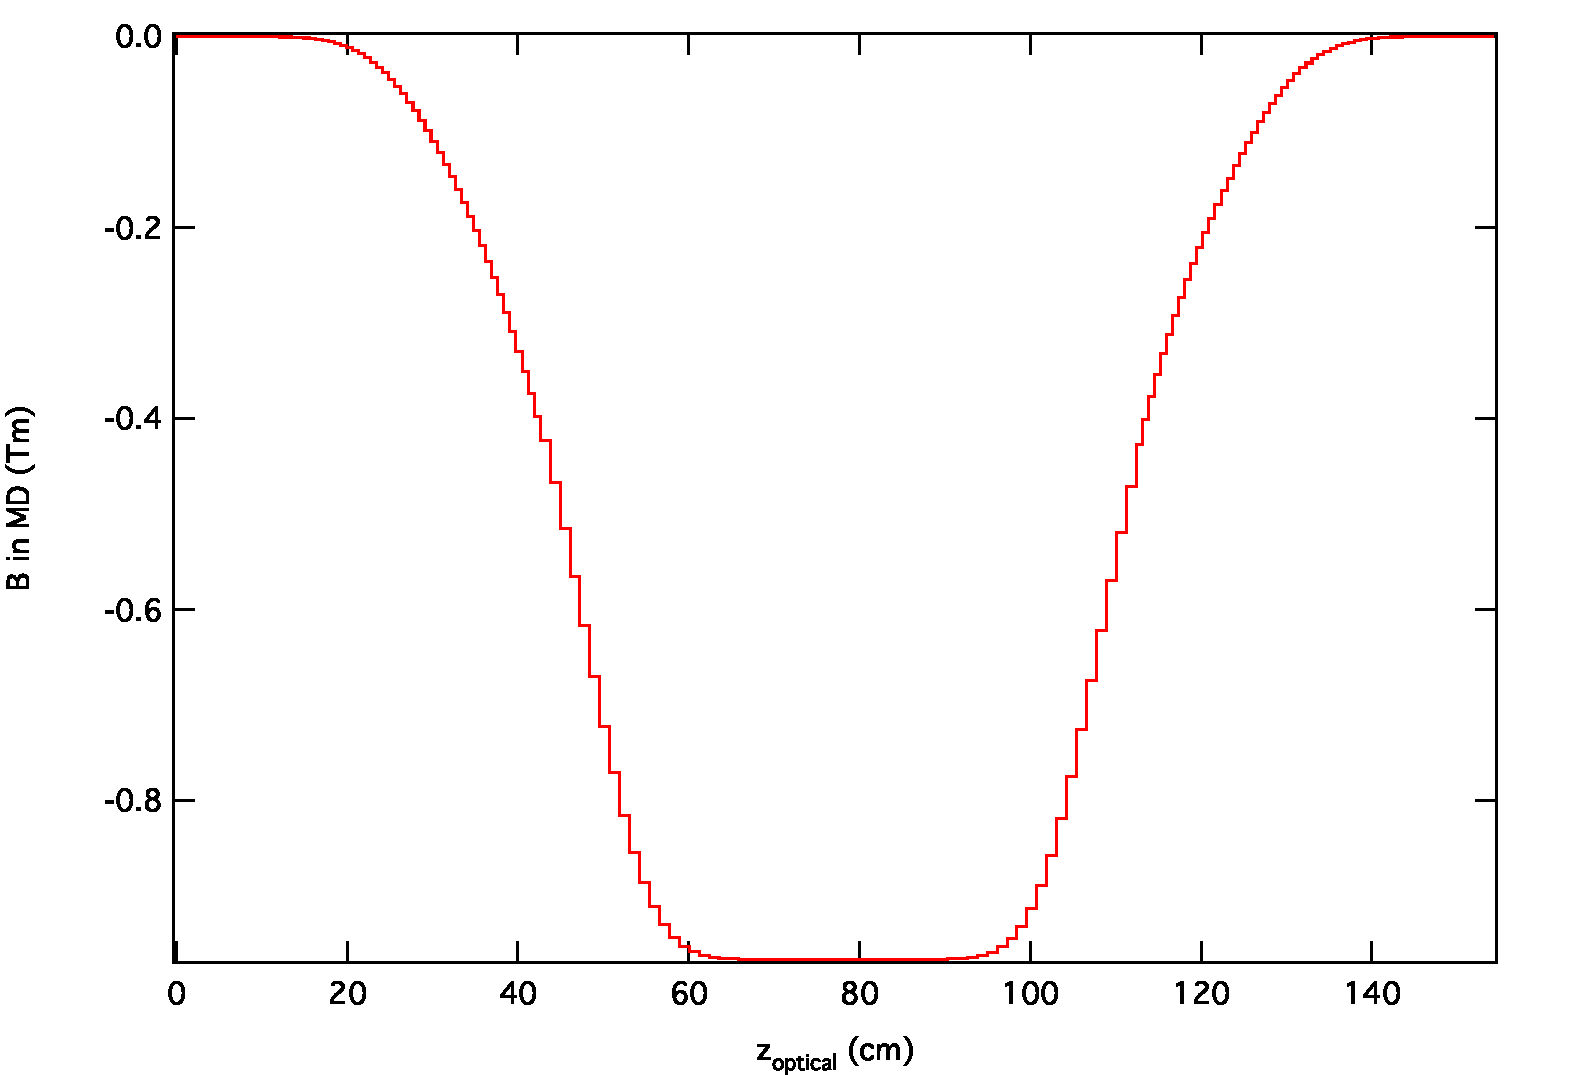
\includegraphics[width=0.5\textwidth]{graphs/MDcutoff}
	}\\
 	\subfloat{
      	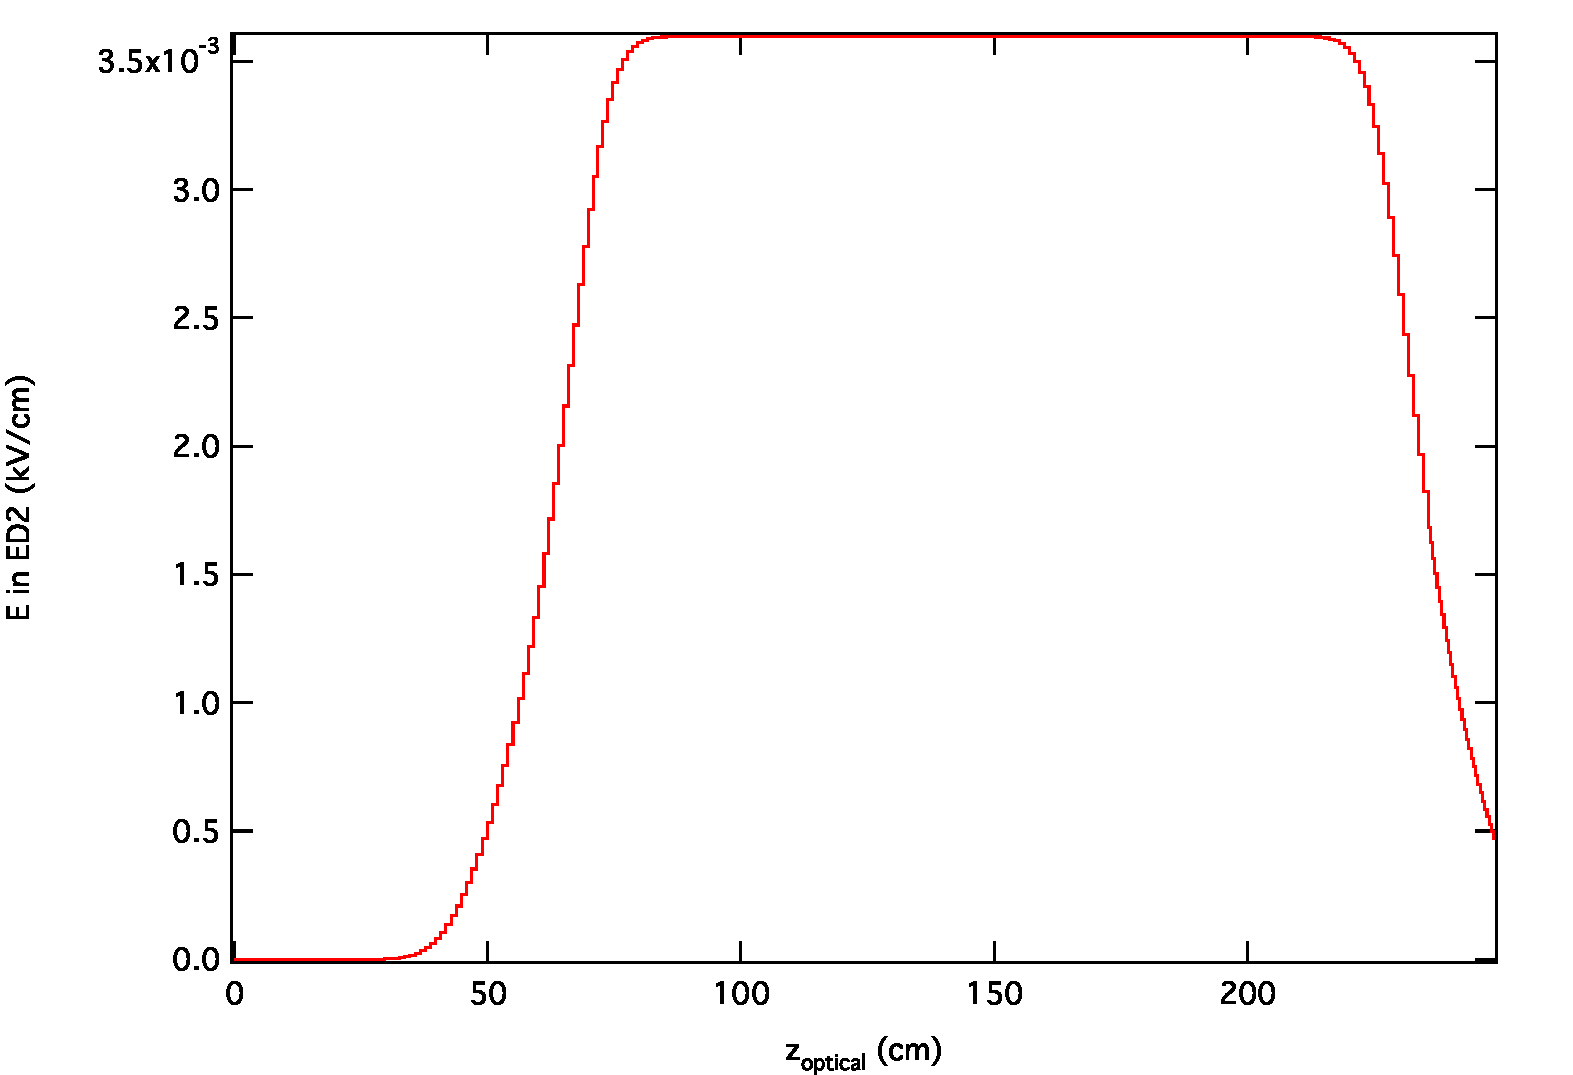
\includegraphics[width=0.5\textwidth]{graphs/ED2cutoff}
	}
	\caption{The change in E and B fields through ED1, MD and ED2 along the optical axis. You can see that the entrance field for ED1 and exit field for ED2 are cutoff.}
	\label{fig:dipoles}
\end{figure}

\subsubsection{To do list}

\textcolor{red}{To do list for the BGField classes:
\begin{enumerate}
\item Change the input EFL of BGField1.cc, BGField2.cc, BGField6.cc and BGField7.cc, for Q1, Q2, Q3 and Q4, such that the output has the desire EFL by printing the fields to file and calculating the output EFL in a separate program (see the Sections \ref{sec:efl} and \ref{sec:eflcalc} on how to do that)
\item ... or better figure out why the output EFL is not the same as the input value. Check the fortran and c++ files in the /fortran/ folder to see if the correct subroutines from \filefont{ray.f} are used to calculate the magnetic quadrupole, magnetic dipole and electric dipole fields. I have not done an fortran-2-c conversions myself so this is something you would have to learn if changes are made in the fortran files.
\item Learn to understand what all the \filefont{data} input parameters mean. Note that different parameters are used for different electric and magnetic elements
\item Figure out why we need to scale B fields by \filefont{userCharge/currentCharge}
\item Add overlapping fields. Field overlaps are not implemented nicely in Geant4 yet. You can figure out a way to nest the BGFieldn.cc classes within each other or read the following reply I got from Peter Gumplinger, a Geant4 specialist at TRIUMF, regarding overlapping fields:\\
{\footnotesize \verbatiminput{inputfiles1.7/GumplingerReply.txt}}
Do this for:
\begin{enumerate}[a]
\item Add overlapping B fields for Q1 and Q2
\item Add overlapping ED1 E field into Q2
\item Add overlapping ED2 E field into Q3
\item Add overlapping B fields for Q3 and Q4
\end{enumerate}
\item Section \ref{sec:useful} has more useful tips on how to debug the E and B fields
\end{enumerate}
}

\subsection{Printing fields to file using EMFieldDebugger.cc}\label{sec:efl}

To calculate the output EFL a new class called EMFieldDebugger.cc was created. This outputs E and B fields of the EDs and MD along the $z_{optical}=0$ optical axis (note that the optical axis curves with the dipoles and is not straight like the z-axis in the world logical volume). The E and B fields are uniform inside EDs and MD. The fields for the quads are zero at $z=0$ and increases radially outward. Therefore the B fields of the quads at a specified radial distance from the optical axis is used. To use EMFieldDebugger.cc change line 1025 in SpectrometerConstruction.cc to\\
\filefont{G4bool calcEFL=TRUE;}\\
This then creates a file named /UserDir/Results/effFieldOpticalAxis.dat and EMFieldDebugger.cc is used. If you want to print the fields of all elements then comment/uncomment lines 1034 to 1039 to look like this:\\
\filefont{      //to calculate fields inside all elements\\
      for(G4int i=0;i<7;i++)\{\\
        EMFieldDebugger* EMdebug = new EMFieldDebugger(i); //writes field strengths at different positions to file\\
      \}\\
      //to calculate field inside one element\\
      //EMFieldDebugger* EMdebug = new EMFieldDebugger(3);}\\
The number $n$ in \filefont{EMFieldDebugger(n)} refers to 0=Q1, 1=Q2, 2=ED1, 3=MD, 4=ED2, 5=Q3, 6=Q4.

If you are working on one element only you can comment/uncomment the lines so that they look like this:\\
\filefont{      //to calculate fields inside all elements\\
      //for(G4int i=0;i<7;i++)\{\\
      //  EMFieldDebugger* EMdebug = new EMFieldDebugger(i); //writes field strengths at different positions to file\\
      //\}\\
      //to calculate field inside one element\\
      EMFieldDebugger* EMdebug = new EMFieldDebugger(3);}\\

There are two parameters that are of particular importance in EMFieldDebugger.cc. The first is \filefont{nn} in line 64. This scales the number of steps decreasing or increasing the step length at which the fields are measured. The larger the number of steps the smaller the step length. You want \filefont{nn=10000}, a large number, to calculate the effective field boundary since the EFL is calculated using a numerical integration (more on this in Sec. \ref{sec:eflcalc}). Any smaller and your results will be affected by the step size. To simply look at the shape of how the field changes as you move into, through and out of the magnet \filefont{nn=3} is sufficient to reduce the number of lines in the file.

To calculate the EFL you need both entrance and exit fringing fields to be complete. Currently the fields for the quads and EDs are cutoff on one end so the tail needs to be artificially completed. If \filefont{transpose = FALSE} (line 65) only the field strengths inside the volumes are printed to file which. The outputs are shown in Fig. \ref{fig:quads} and \ref{fig:dipoles}. Since the fields are symmetric around the center you can transpose the field from one tail to the other. If you set it to \filefont{transpose = TRUE} both tails are complete, as shown in Fig. \ref{fig:quads2} Fig. \ref{fig:ed2}. You can use the /UserDir/Results/effFieldOpticalAxis.dat file to calculate the effective field boundaries and hence the effective field lengths with EFLcalculator.cc. This is a separate c++ routine to gemma1.7 described in Sec. \ref{sec:eflcalc}.

\begin{figure}
\centering
 	\subfloat{
      	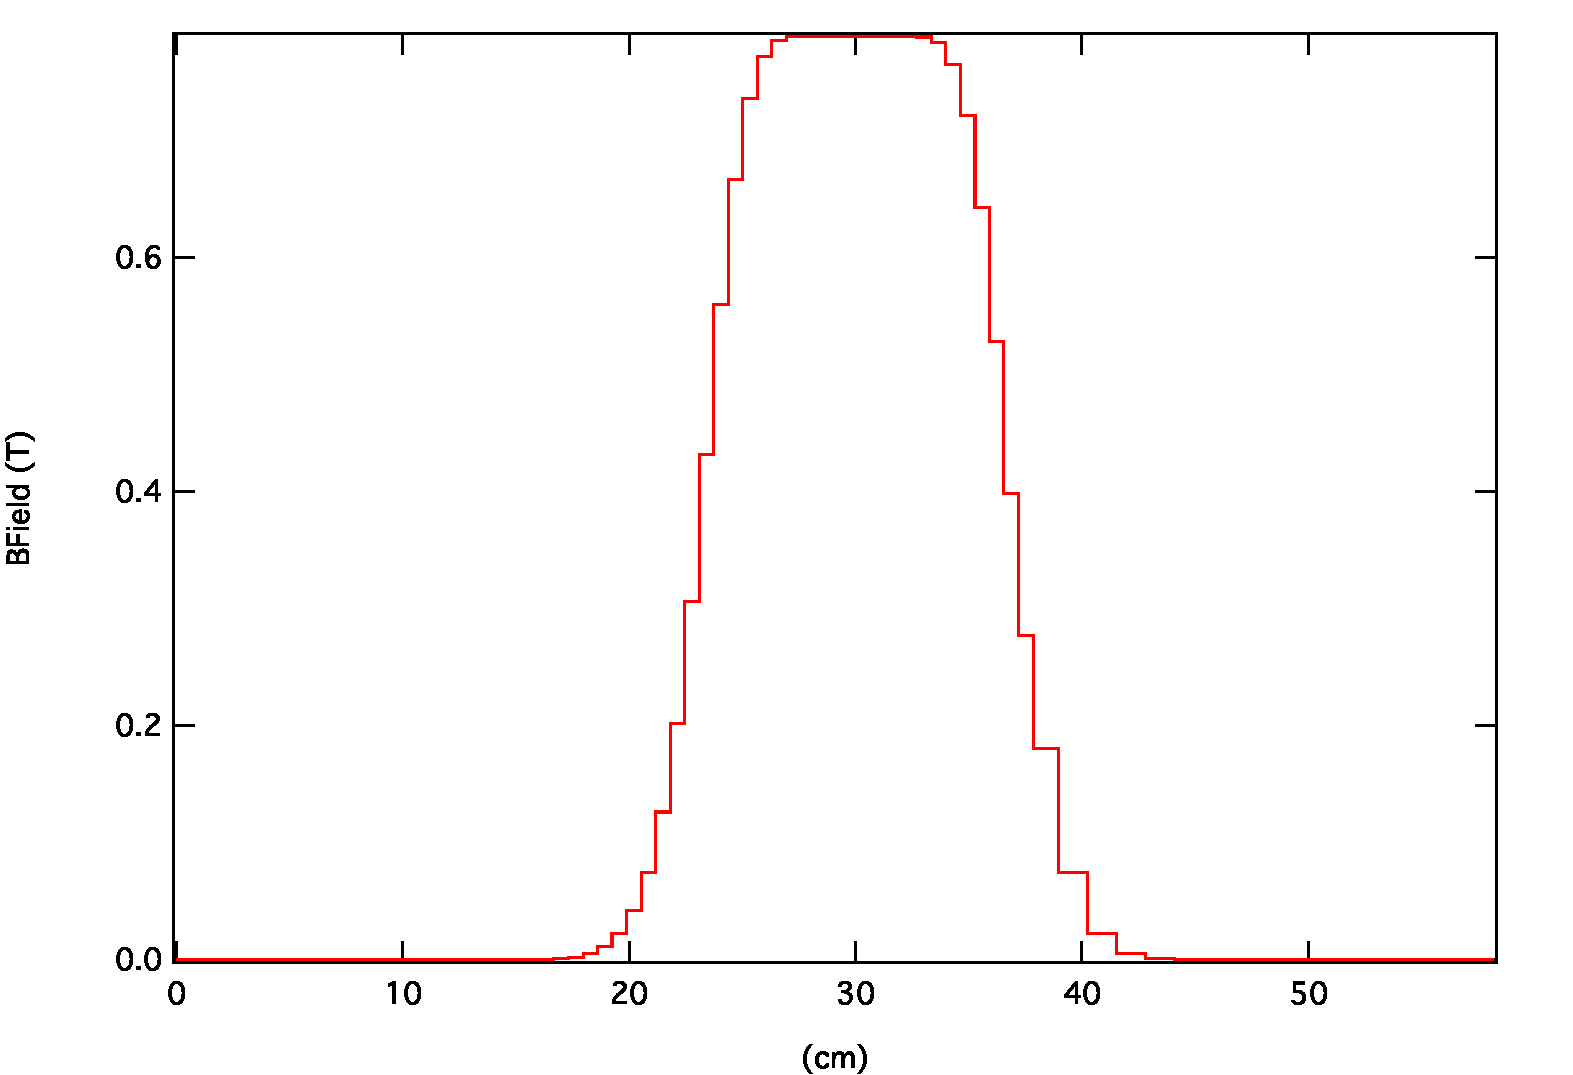
\includegraphics[width=0.5\textwidth]{graphs/Q1complete}
	}
	\subfloat{
	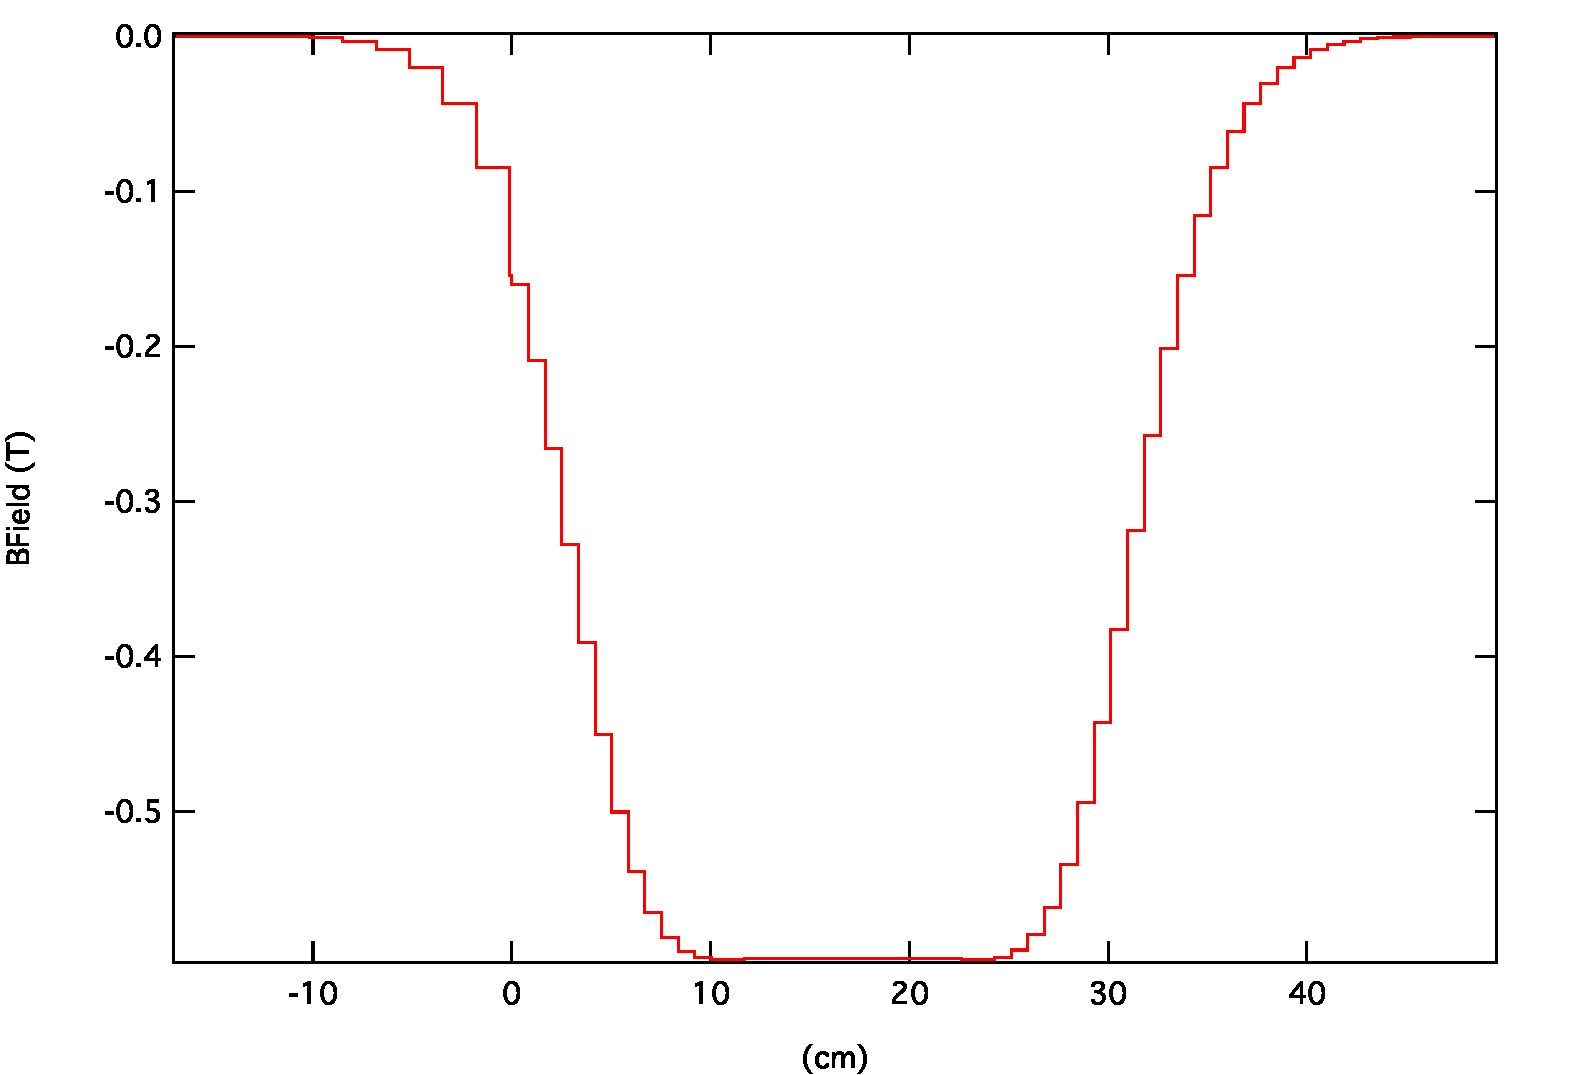
\includegraphics[width=0.5\textwidth]{graphs/Q2complete}
	}\\
 	\subfloat{
      	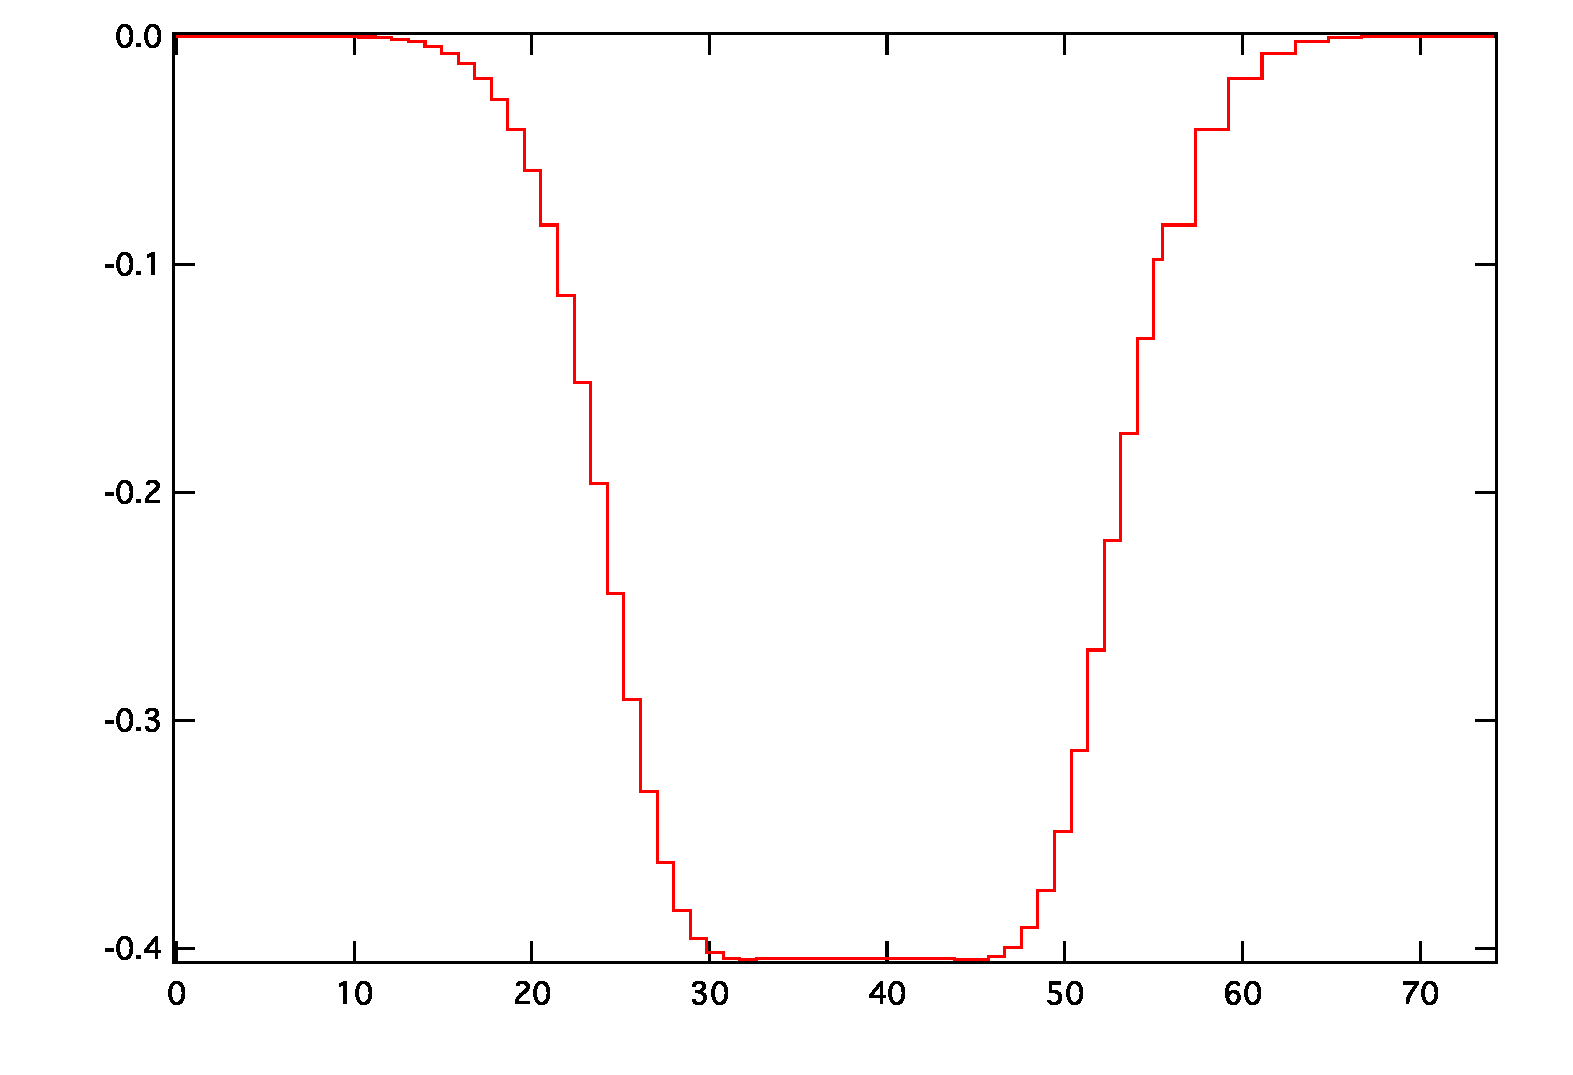
\includegraphics[width=0.5\textwidth]{graphs/Q3complete}
	}
	\subfloat{
	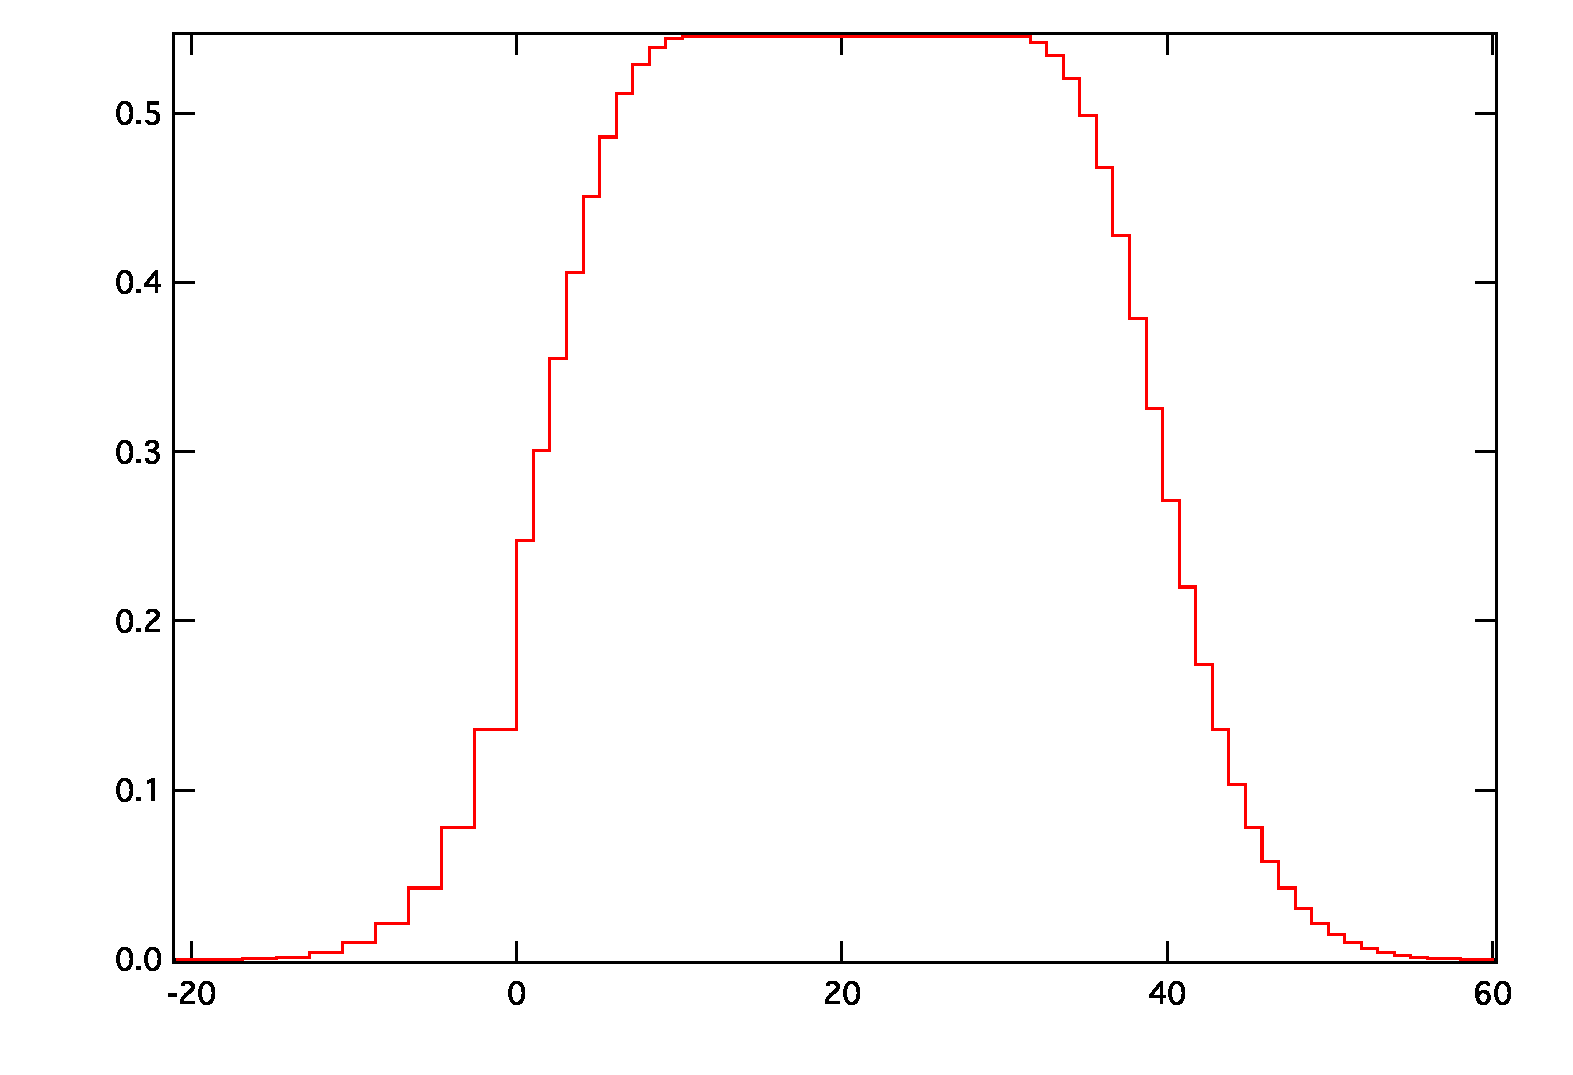
\includegraphics[width=0.5\textwidth]{graphs/Q4complete}
	}
	\caption{The change in B field through Q1, Q2, Q3 and Q4 with the cutoff tails artificially completed.}
	\label{fig:quads2}
\end{figure}

\begin{figure}
\centering
 	\subfloat{
      	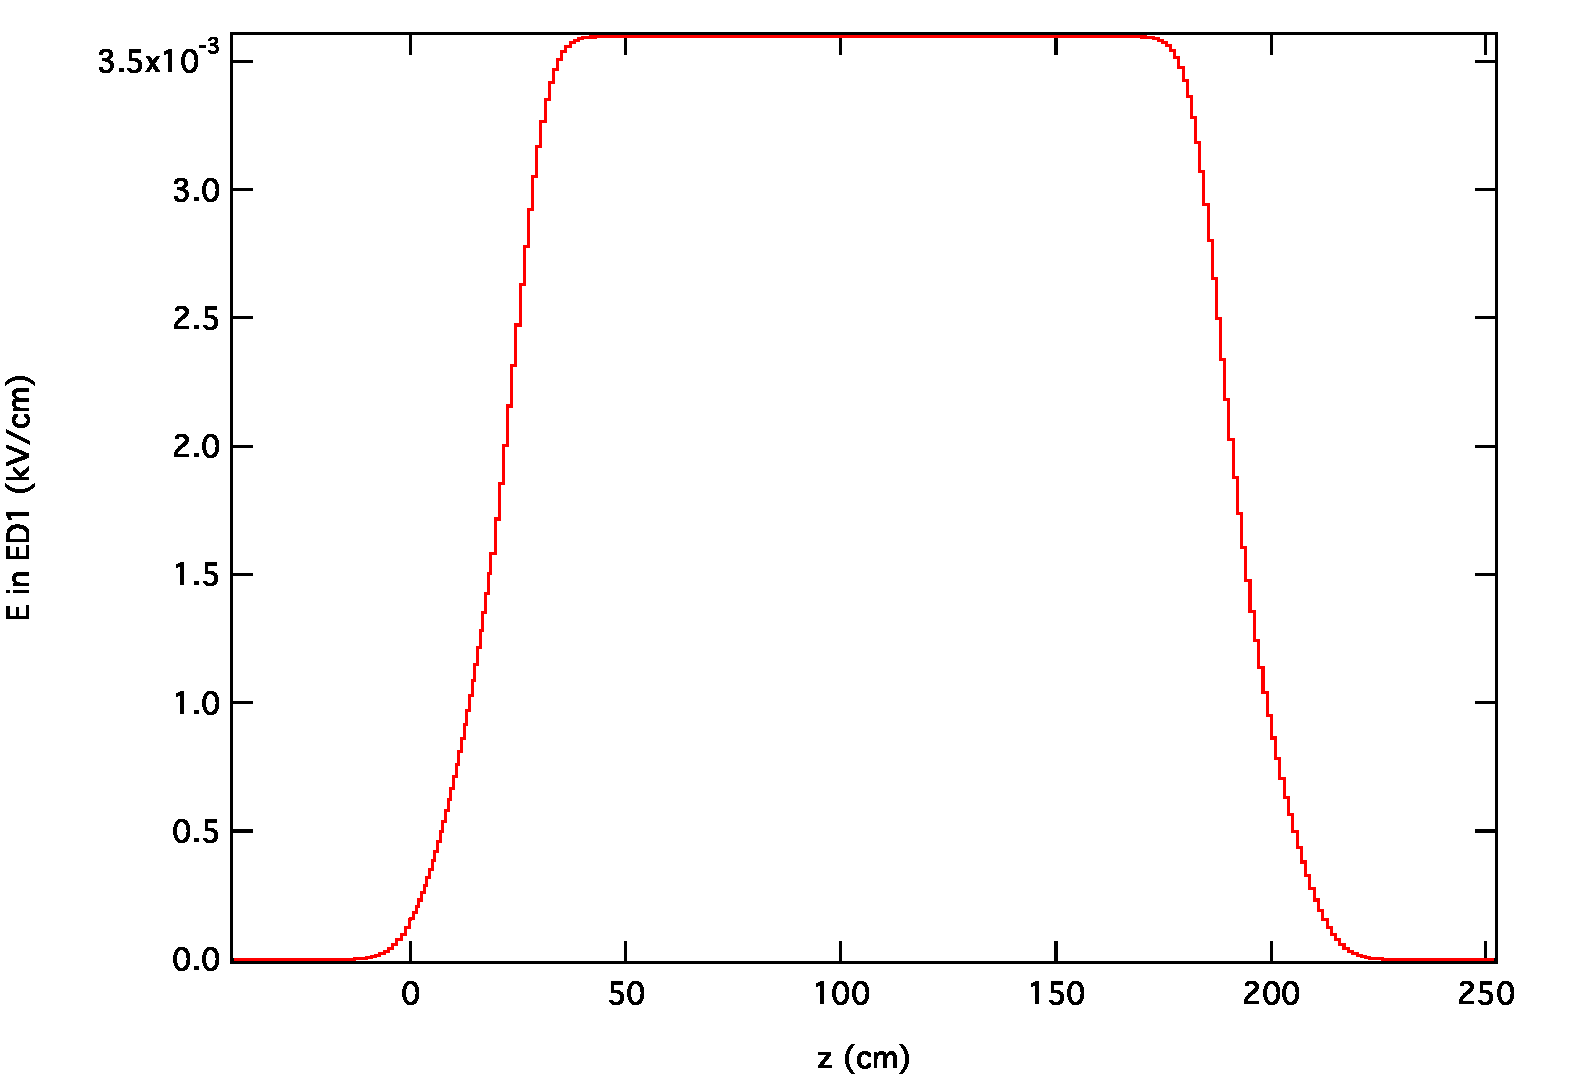
\includegraphics[width=0.5\textwidth]{graphs/ED1complete}
	}
	\subfloat{
	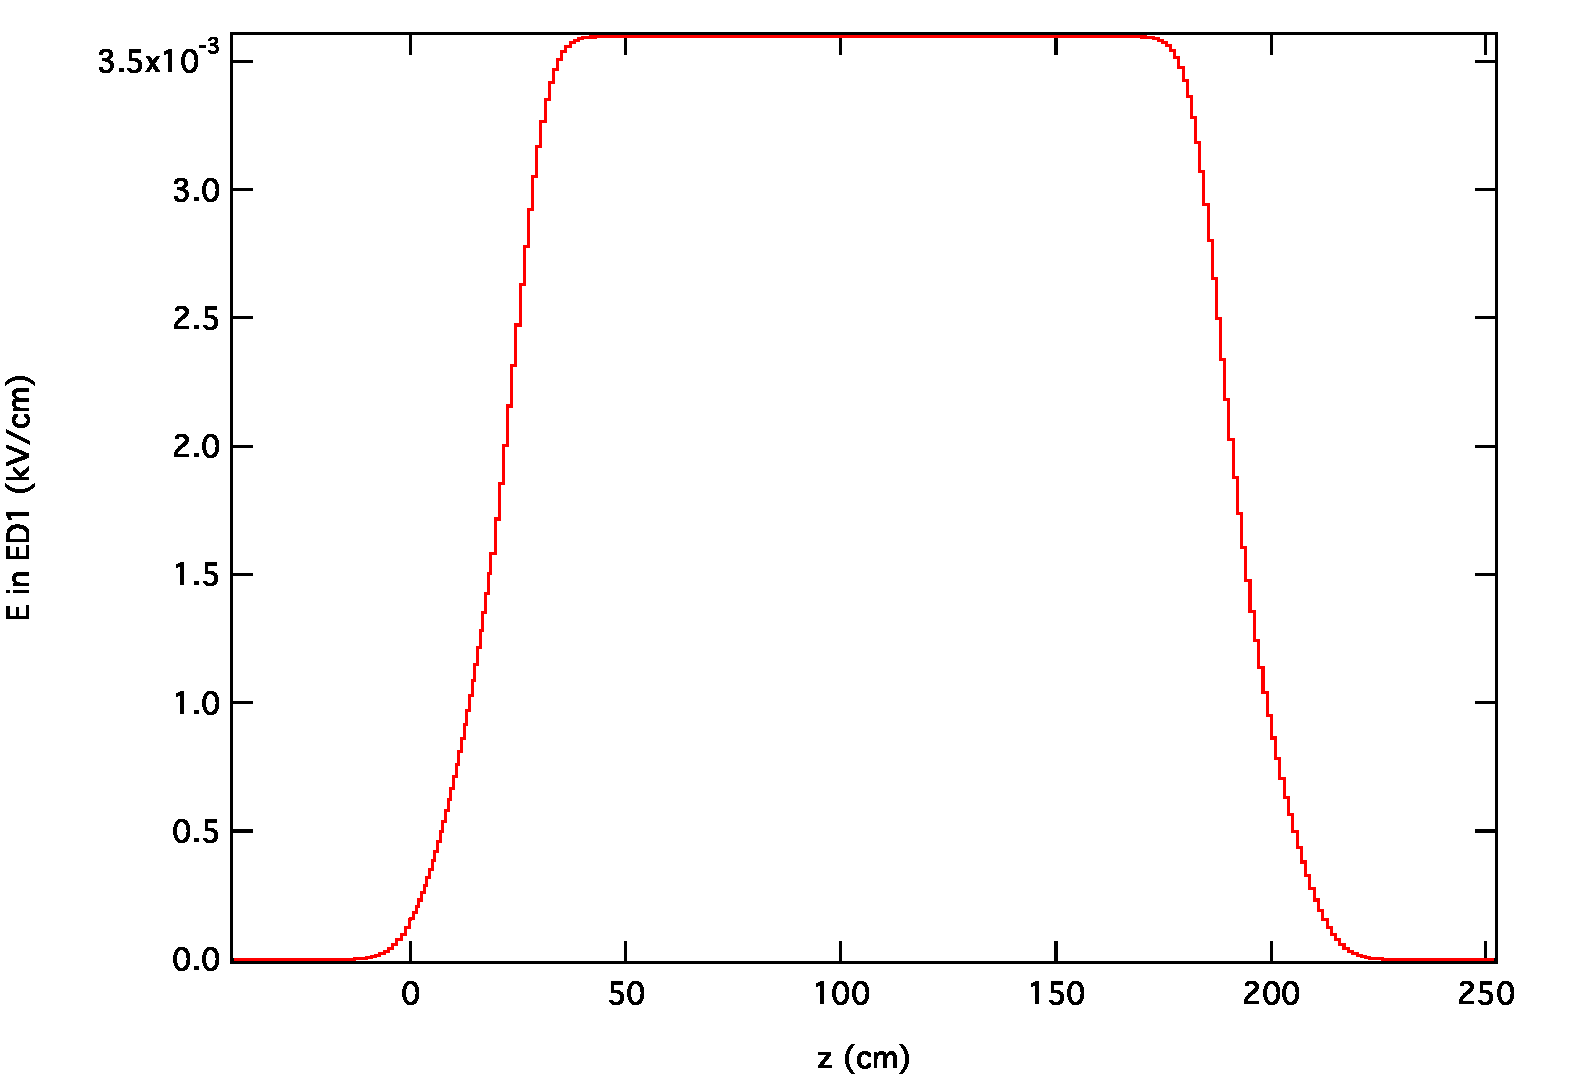
\includegraphics[width=0.5\textwidth]{graphs/ED1complete}
	}\\
	\caption{The change in E field through ED1 and ED2 with the cutoff tails artificially completed.}
	\label{fig:ed2}
\end{figure}


Note:
\begin{itemize}
\item Do not take the field values calculated with EMFieldDebugger.cc in SpectrometerConstruction.cc to be the actual field values. Where it is used in SpectrometerConstruction.cc the \filefont{FieldStrength\_0} in the BGField.cc has not been scaled yet nor have the \filefont{userCharge} and \filefont{currentCharge} been changed to equal that of the simulated particle. 
\item If you want to print out the actual field strengths I suggest you implement EMFieldDebugger.cc in EMMASteppingAction.cc. A convenient place to put it is in the debugging section after line 295 in the UserSteppingAction(const G4Step* theStep) object of EMMASteppingAction.cc.
\item The fields of Q1, Q2, Q3 and Q4 are obtained at r=2, 5, 5 and 7 cm respectively. These are arbitrarily selected radial distances. The condition to chose a radius is that it's bigger than 0 and smaller than the poll tip radius (\filefont{data[12]} in BGFieldn.cc).
\item If you change the dimensions of the volumes containing the fields in SpectrometerConstruction.cc make sure the correct lengths are passed through to EMFieldDebugger.cc.
\end{itemize}

\subsection{Calculating the output EFL using EFLcalculator.cc}\label{sec:eflcalc}

If you set \filefont{nn=10000} and \filefont{transpose = TRUE} in EMFieldDebugger.cc you can use the output file /UserDir/Results/effFieldOpticalAxis.dat to calculate the effective field lengths using EFLcalculator.cc found in the folder /UserDir/Results/fringefields/.

Compile EFLcalculator.cc using the command:\\
\filefont{g++ EFLcalculator.cc -o EFLcalculator}\\
and run the program using the command:\\
\filefont{./EFLcalculator effFieldOpticalAxis.dat}

The fringing fields, i.e. the entrance and exit fields, have a slope as can be seen in Fig. \ref{fig:quads} and Fig. \ref{fig:dipoles}. However, you can describe the fringe field as having a sharp boundary. The effect on the particle is the same whether you have a gradually increasing fringing field or a constant field starting at the sharp boundary. This is boundary is called the effective field boundary. This is illustrated in Fig. \ref{fig:EFB}.

In the dipoles the field is uniform between the poles and therefore the particle feels the same field $B_{0}$ everywhere in between the ED and MD. In the quads the field is constant parallel to the optical axis but changes linearly perpendicularly to it. It is zero at the center and linearly increases radially outwards with a maximum field at the poll tips. Therefore the gradient of the field is used 
\begin{equation}
g=B(r)/r
\end{equation}
where $r$ is the radial distance perpendicular from the optical axis and $B(r)$ is the magnetic field strength at that radius.

\begin{figure}
\centering
 	\subfloat[]{
      	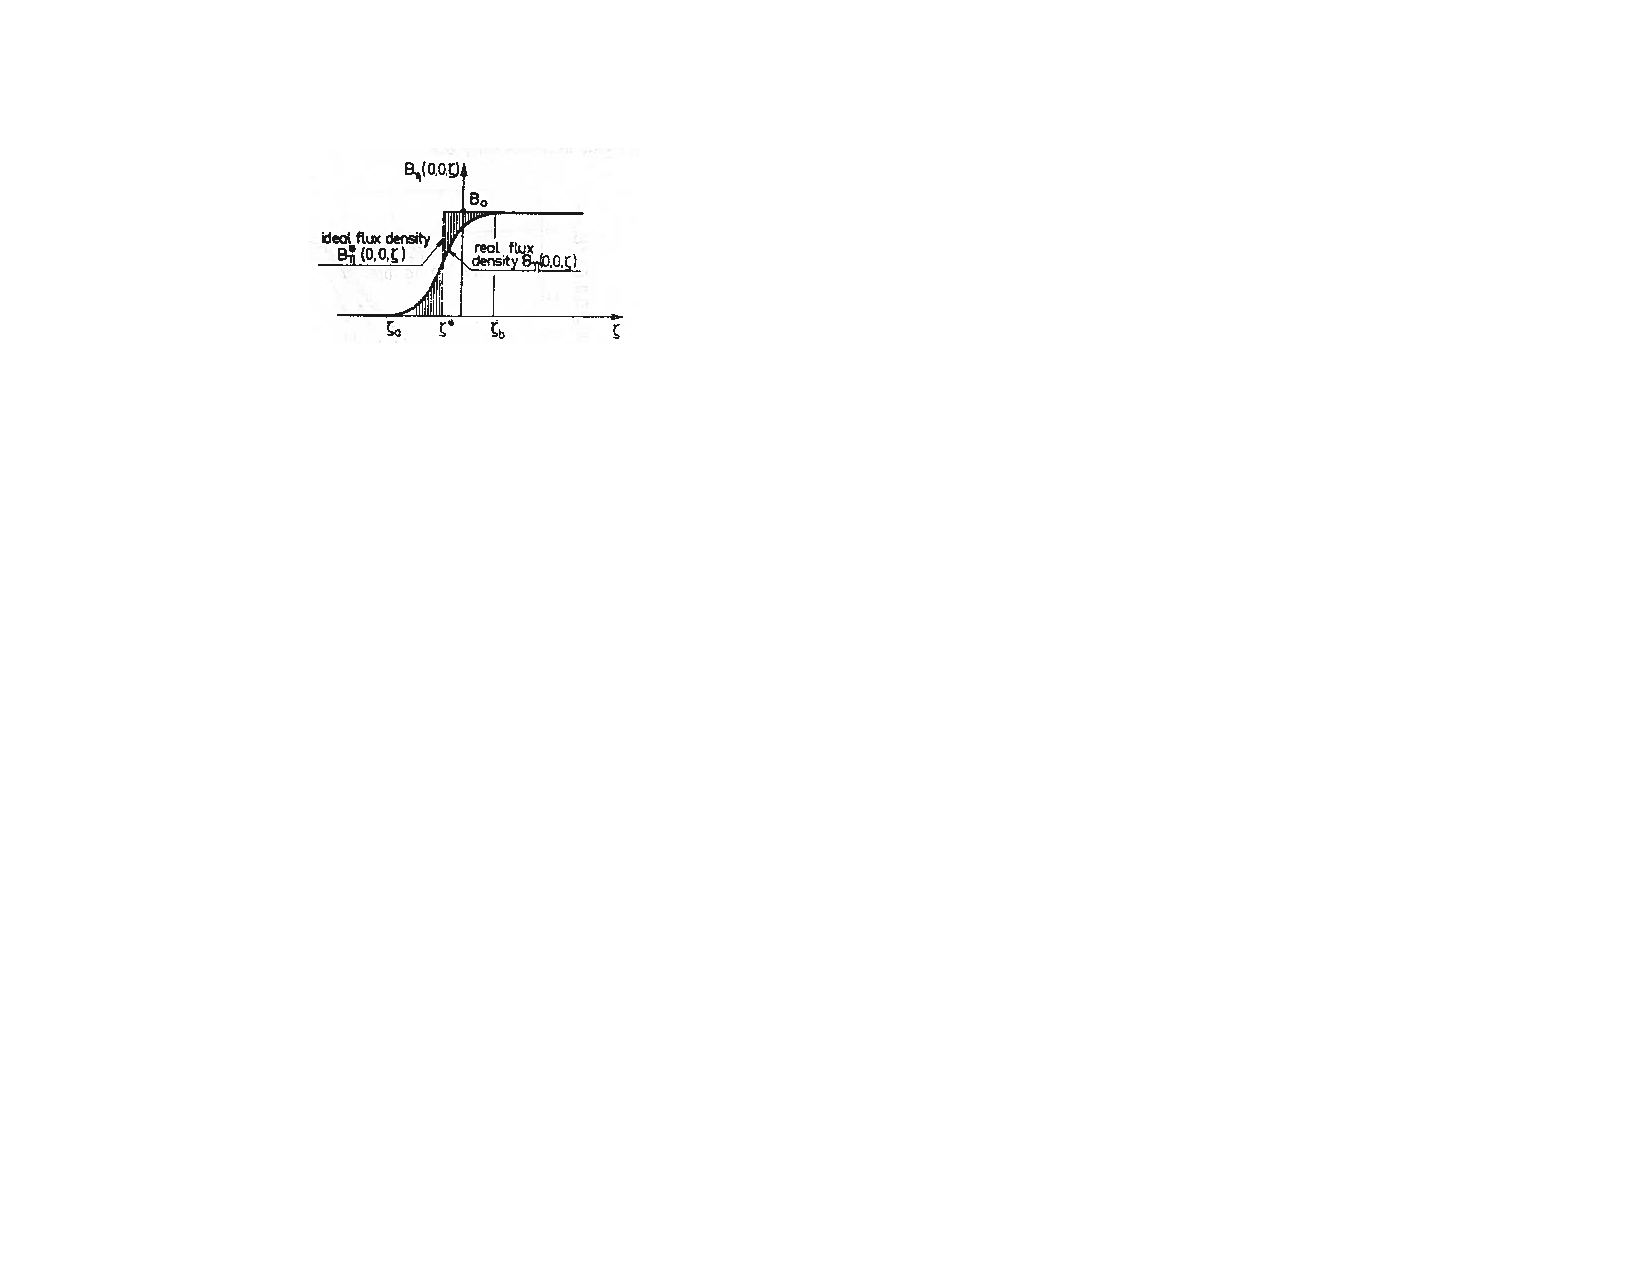
\includegraphics[width=0.5\textwidth]{graphs/EFBdipole}
	}
	\subfloat[]{
	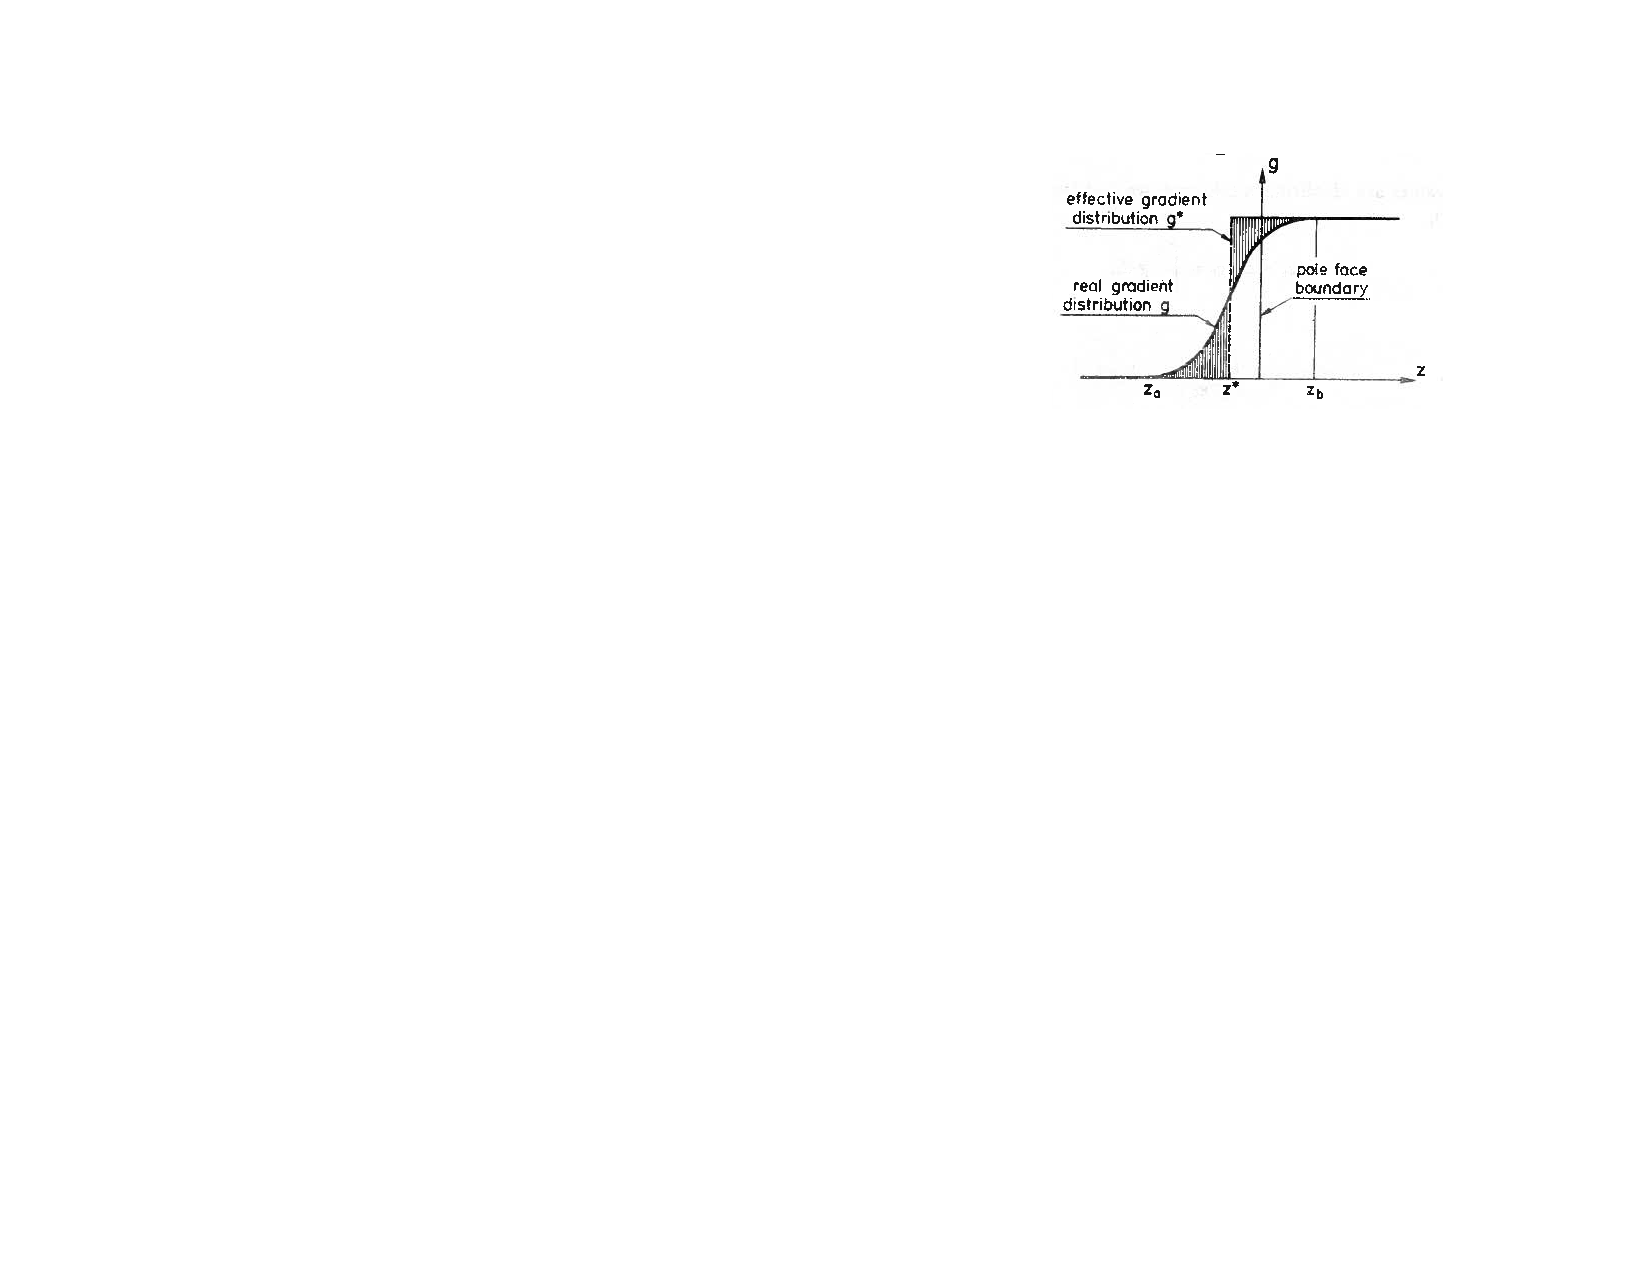
\includegraphics[width=0.5\textwidth]{graphs/EFBquad}
	}
	\caption{(a) The distribution of the fringing field $B(\zeta)$ and and the effective field boundary $\zeta^{*}$ for the dipoles. $\zeta$ is the distance along the optical axis. $B_{0}$ is the constant field strength after $\zeta_{b}$ where the constant field begins. The field starts at $\zeta_{a}$. (b) The distribution of the gradient of the fringing field $g(z)$ and and the effective field gradient boundary $z^{*}$ for the quads. $z$ is the distance through the quadrupole but at a radial distance $r$ from the optical axis. In my calculations $\zeta$ and $z$ are the same thing. (Taken from 'The Optics of Charged Particles' by Wollnik, Hermann)}
	\label{fig:EFB}
\end{figure}

To calculate $z^{*}$, the effective field boundary, the following integrals are used for the electric dipoles, magnetic dipoles and the magnetic quads:
\begin{align}
z^{*}=z_{b}-\int^{z_{b}}_{z_{a}}\frac{E(z)}{E_{0}}dz\label{eq:integral1}\\
z^{*}=z_{b}-\int^{z_{b}}_{z_{a}}\frac{B(z)}{B_{0}}dz\label{eq:integral2}\\
z^{*}=z_{b}-\int^{z_{b}}_{z_{a}}\frac{g(z)}{g_{0}}dz\label{eq:integral3}
\end{align}
where $z_{a}$ is any location outside the volume where the field is zero and $z_{b}$ where the field becomes constant. $E$, $B$ and $g$ are the electric field, magnetic field and the magnetic field gradient. $E(z)$, $B(z)$ and $g(z)$ are the field strengths/gradients as a function of $z$ and $E_{0}$, $B_{0}$ and $g_{0}$ are the constant field strengths/gradients. 

EFLcalculator.cc finds $z_{b}$ for the entrance and exit fringing fields and does the integrals in Eq. \ref{eq:integral1} to \ref{eq:integral3} numerically. The effective field length is then the difference between the exit and entrance effective field boundary
\begin{equation}
EFL=z^{*}_{exit}-z^{*}_{entrance}
\end{equation}

If you run the code an output file named FFIntegrals.dat is generated with the EFL for each electric and magnetic element. I am confident the numerical integrals are done right in the code. I checked it with a known distribution. As long as \filefont{nn=10000}, \filefont{transpose = TRUE} in EMFieldDebugger.cc the results can be trusted.

You want these output EFLs to be that of the specified values listed in Table \ref{tab:desiredefl}. Here is the procedure of how to achieve this:
\begin{enumerate}
\item In SpectrometerConstruction.cc set:\\
\filefont{G4bool calcEFL=TRUE;} line 1027\\
uncomment\\
\filefont{exit(0);} line 1042 (this terminates ./EMMAapp after it prints the fields to file)\\
and either use:\\
\filefont{      //to calculate fields inside all elements\\
      for(G4int i=0;i<7;i++)\{\\
        EMFieldDebugger* EMdebug = new EMFieldDebugger(i);\\
      \}
      }\\
or\\
\filefont{        //to calculate field inside one element\\
      EMFieldDebugger* EMdebug = new EMFieldDebugger(n);}\\
The number $n$ in \filefont{EMFieldDebugger(n)} refers to 0=Q1, 1=Q2, 2=ED1, 3=MD, 4=ED2, 5=Q3, 6=Q4.
\item Set \filefont{nn=10000} and \filefont{transpose = TRUE} in EMFieldDebugger.cc
\item\label{it:change} Change \filefont{data[11]} for the quads in BGField1, 2, 6 and 7.cc and change \filefont{data[15]} for the EDs and MD in BGField 3, 4 and 5.cc
\item Compile gemma1.7 with \filefont{make}
\item Run gemma1.7 with \filefont{./EMMAapp}. This should terminate on its own since you have the \filefont{exit(0)} statement in SpectrometerConstruction.cc right after the fields are written to file.
\item A file calle effFieldOpticalAxis.dat is produced which you will use as the input file to EFLcalculator.cc. This routine automatically finds the words ``Q1'', ``Q2'', etc in the file so it doesn't matter if the fields of only one, two, or all elements are in this data file and what order they are in. Run the routine using:\\
\filefont{./EFLcalculator effFieldOpticalAxis.dat}
\item\label{it:ouput} Use the output values in the terminal or EFLcalculator.cc to determine the EFL calculated by the BGFieldn.cc
\item Repeat point \ref{it:change} to \ref{it:ouput} till desired output EFL is achieved
\end{enumerate}



\begin{table*}
\caption{Effective field length (EFL) inputs}\label{tab:desiredefl}
\centering
\begin{threeparttable}
\begin{tabular}{cccc}
\hline
	&EFL (cm)	&Radius (cm)	&Angle specification (deg)	\\
\hline
Q1	&13.977		&&\\
Q2	&29.88		&&\\
ED1	&174.533\tnote{a}	&500			&20\\
MD	&69.813\tnote{a}	&100			&40\\
ED2	&174.533\tnote{a}	&500			&20\\
Q3	&29.88		&&\\
Q4	&40.18		&&\\
\end{tabular}
     \begin{tablenotes}
       \item[a] {\small Eq. \ref{eq:eflcurve} was used to calculated these.}
     \end{tablenotes}
\end{threeparttable}
\end{table*}

\subsubsection{To do list}

\textcolor{red}{To do list to calculate output EFL and use it as BGField.cc inputs:
\begin{itemize}
\item Follow above instructions to acquire correct output EFL for Q1, Q2, ED1, MD, ED2, Q3 and Q4
\item If instead you are fixing the BGField.cc classes and want to check the output EFL follow the same instructions except leave out point \ref{it:change}
\end{itemize}
}


\subsection{Useful things to do when debugging the E and B fields}\label{sec:useful}

When you are debugging the E and B fields you might want to change the /userDir/UserInput/beam.dat file so that it contains
{\footnotesize \verbatiminput{inputfiles1.7/beam.dat}}
and the /userDir/UserInput/centralTrajectory.dat to
{\footnotesize \verbatiminput{inputfiles1.7/centralTrajectory.dat}}
This means that if you start \filefont{./EMMAapp} and run the command:
\filefont{/mydet/doBeam}
you will shoot only one particle with Z=50, A=133, Q=30 and E=258 MeV. The centralTrajectory.dat file is used to scale the E and B fields of all the elements to the specified reference particle. Sine, in this case, the beam particle is the same as the reference particle the beam should hit the focal place at $(x,y)=(0,0)$. The screen output when shooting a beam particle with these input files is currently:\\

\filefont{Prim.Gen.Action output Energy(MeV)= 258 z emission location (mm) -1.5e-06 theta(deg)= 0 phi(deg)= 0\\
Start event: 0\\

	>>> Event 0 >>> Simulation truth : Sn133[0.0] (0,0,7996.4634352405)\\
Stopping Block has 425 hits.\\
	Focal Plane (x,y) -5.1294024872165, 0 mm.\\
	Ekin 258.06662284817 MeV\\}
	
The second to last line indicates that this beam particle hits the focal plane at (x,y)=(-5.1 mm,0). This is an indicator that BGFieldn.cc calculate the wrong fields. The wrong fields, especially for the ED1, MD and ED2, even at a 0.1\% difference, make a big difference.

The top line of the screen output is created in line 260 of EMMAPrimaryGeneratorAction.cc:\\
\filefont{    G4cout<<"Prim.Gen.Action output "<<"Energy(MeV)= "<<energy <<" z emission location (mm) "
          <<zemit/mm<<" theta(deg)= "<<theta/deg<<" phi(deg)= "<<phi/deg<<G4endl;}


The energy of the particle is set to be monoenergetic for all particles. If you want to add the beam energy uncertainty change lines 205 to 210 as needed\\
\filefont{//---------------------------------------------------------------------------------------//\\
    //energy including spread\\
    //particleGun->zSetParticleEnergy(Ekin *MeV);\\
    //fixed energy\\
    particleGun->SetParticleEnergy(energy *MeV);\\
//---------------------------------------------------------------------------------------//\\}

The z emission location $z_{emission}$ is where the particle starts. $z$=0 is defined to be the center of the target. $z_{emission}$ is currently set to be 10 Ang before the target. Currently $x_{emission}=0$ and $y_{emission}=0$. This can be changed in lines 223 to 228:\\
\filefont{//---------------------------------------------------------------------------------------//\\
    //random emittance off optical axis\\
    //particleGun->SetParticlePosition(G4ThreeVector(xBeam,yBeam,zemit));\\
    //fix emittance location to optical axis\\
    particleGun->SetParticlePosition(G4ThreeVector(0,0,zemit));\\
//---------------------------------------------------------------------------------------//\\}

The emission angle is set to 0 deg. This can be changed in lines 243 to 262:\\
\filefont{//---------------------------------------------------------------------------------------//\\
    //random angles\\
    /*if (MaxAngle>0.) \{\\
      G4double theta = G4UniformRand() * MaxAngle * sqrt(1.0-(r/rmax)*(r/rmax));\\
      G4double phi = G4UniformRand()*CLHEP::twopi;\\
      x = sin(theta) * cos(phi);\\
      y = sin(theta) * sin(phi);\\
      z = cos(theta);\\
    \}*/\\
    //fixed angles\\
    G4double theta = 0*deg;\\
    G4double phi = 0*deg;\\
    x = sin(theta) * cos(phi);\\
    y = sin(theta) * sin(phi);\\
    z = cos(theta);\\
    particleGun->SetParticleMomentumDirection(G4ThreeVector(x,y,z));\\
    
    G4cout<<"Prim.Gen.Action output "<<"Energy(MeV)= "<<energy <<" z emission location (mm) "\\
          <<zemit/mm<<" theta(deg)= "<<theta/deg<<" phi(deg)= "<<phi/deg<<G4endl;\\
//---------------------------------------------------------------------------------------//\\}

I would keep it as it is till you end up with the Z=50, A=133, Q=30 and E=258 MeV beam particle hitting the focal plane close to $(x,y)=(0,0)$

Once this is achieved you can maybe try shooting the beam particle at an angle of $(\theta,\phi)=(2 deg,0)$. This will shoot the particle at 2 deg to the x-axis. You can then compare the x and y positions along the optical plane at the exits of all electric and magnetic elements with Barry Davids' ion optics code outputs. In EMMASteppingAction.cc you can print out the positions of the particles at each step. Below line 295 this class prints out the x and y positions wrt to the optical axis at the exits of each magnetic for each electric element for each particle. Since the ion optics code uses the optical axis the $z_{optical}$ axis will bend with the EDs and MD. Since the dimensions have recently changed you will need to recalculated the equation of plane at the end of the ED1 and MD boundaries to acquire the x and y exit positions wrt optical axis. The equation of plane is
\begin{equation}
ax+by+cz=-d
\end{equation}
Fig. \ref{fig:plane} should contain all the necessary parameters to calculate the coefficients $a$, $b$, $c$ and $d$. Then make the necessary changes between lines 327 and 355 in EMMASteppingAction.cc.

\begin{figure}
\centering
 	\subfloat[]{
      	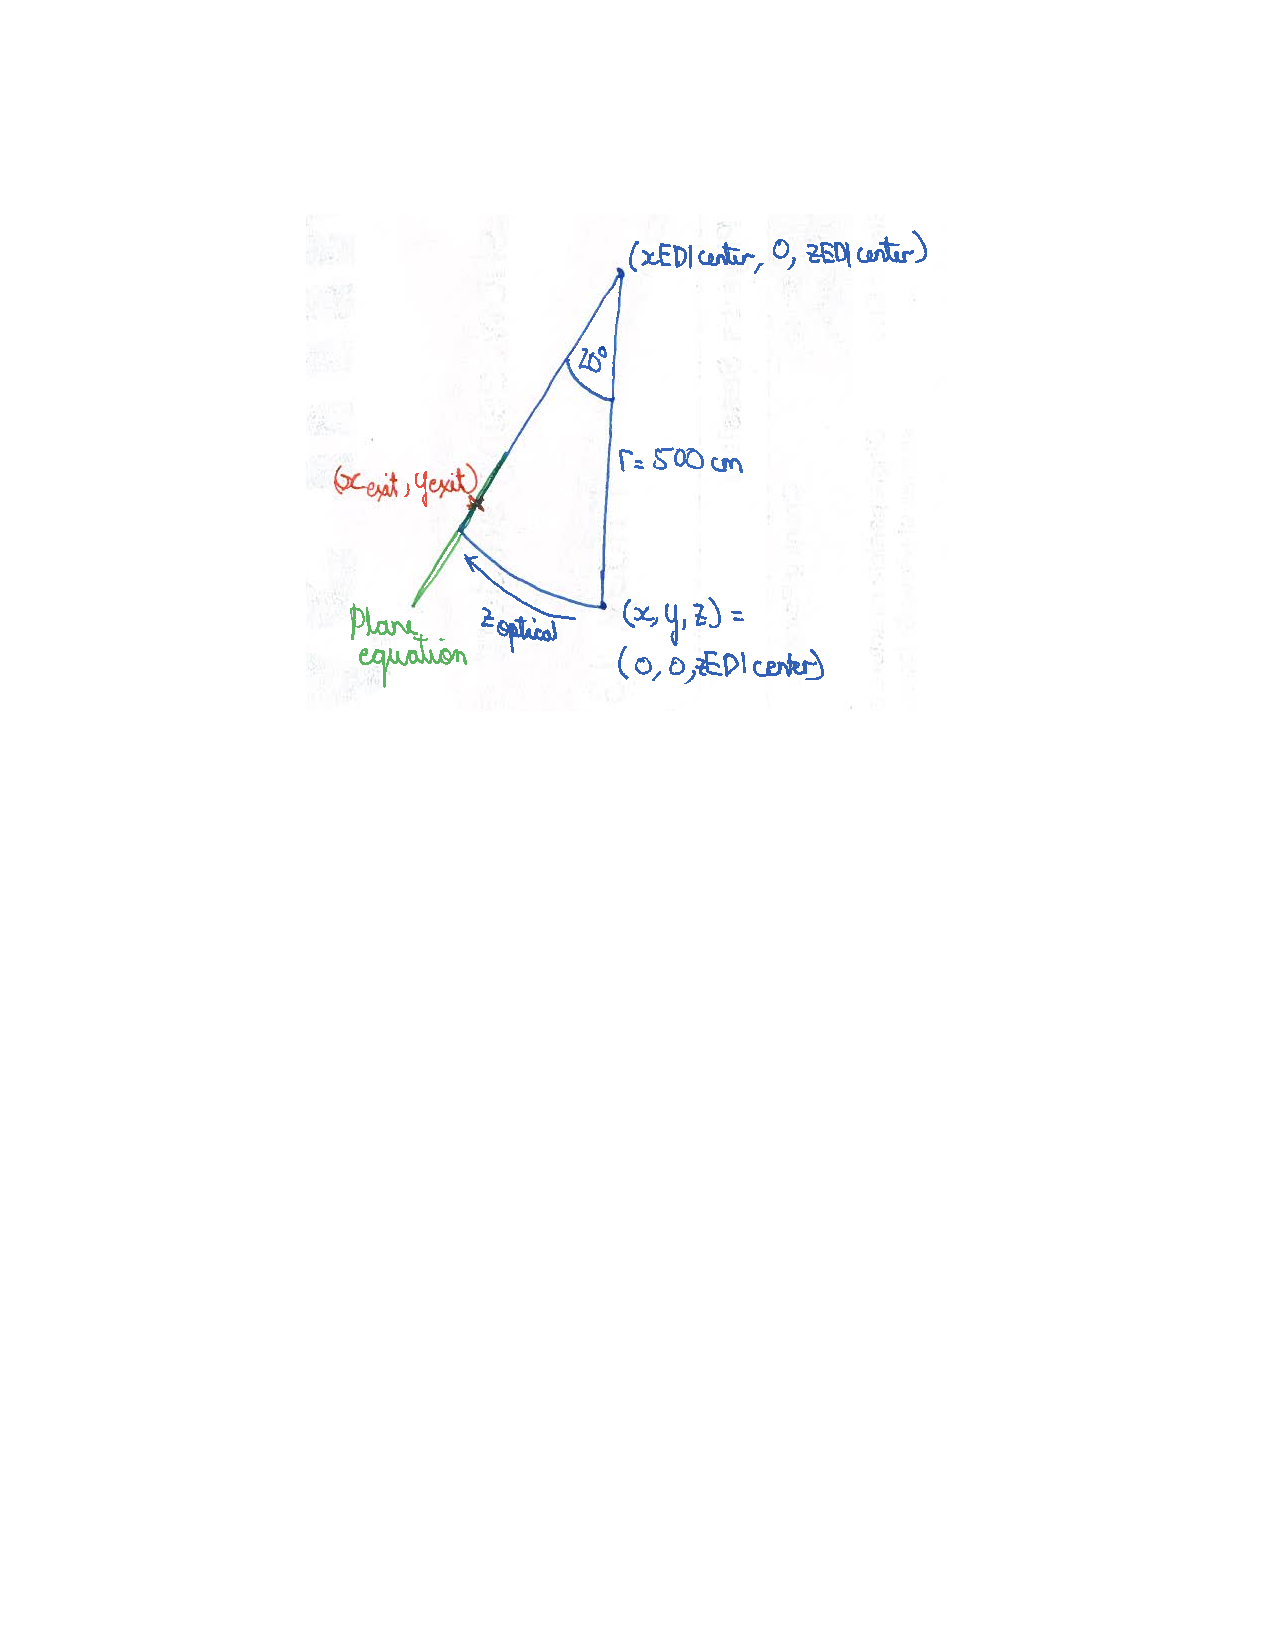
\includegraphics[width=0.5\textwidth]{graphs/planequationED1}
	}
	\subfloat[]{
	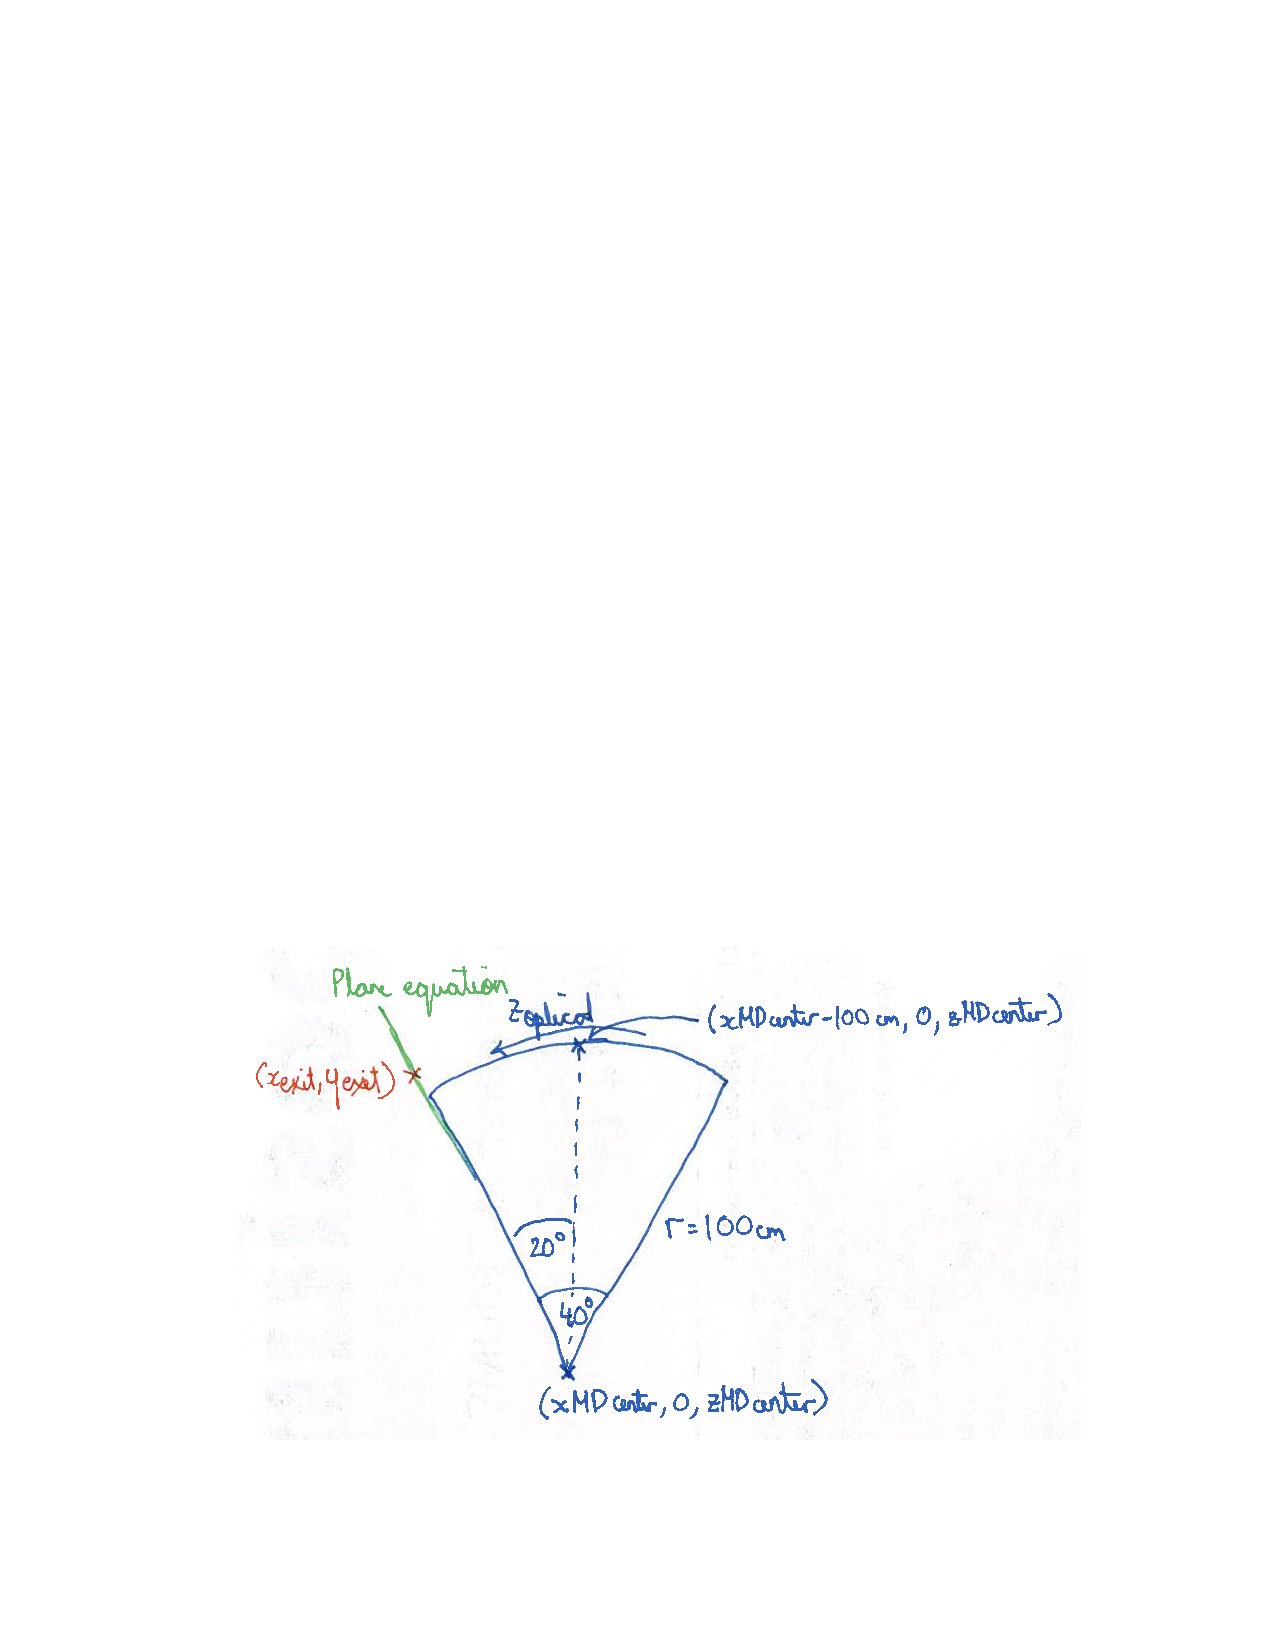
\includegraphics[width=0.5\textwidth]{graphs/planequationMD}
	}
	\caption{Parameters needed to calculate the plane of equation at the exit of (a) ED1 and (b) MD. $(x_{exit},y_{exit})$ (in red) is what you want to compare with Barry's ion optics code. All positions in written in blue are variables defined in SpectrometerConstruction.cc, which you should print out to find it's numerical value.}
	\label{fig:plane}
\end{figure}

\subsection{ROOT analysis}

I have changed the the root analysis macros located in /userDir/Results/rootanalysis slightly. There are now two macros called GEMMArootanalysis\_v1.C and GEMMArootanalysis\_v2.C. GEMMA1.6documentation.pdf doesn't explain the root file in much detail, so I'll do that here. 

Two histograms called ``hitpos'' and ``hitangle'' are created in EMMAEventAction.cc. hitpos is a 2D histogram that stores the x and y hit position of the particles at the focal plane. hitangle is a 1D histogram that stores the angle of the particles to the focal plane. In EMMASteppingAction.cc a 1D hisogram called ``dead\_hit'' is created. If a particle hits a wall or a slit and is terminated then the name of the wall or slit is stored in this histogram. If you want to view these histograms use GEMMArootanalysis\_v1.C:\\
\begin{enumerate}
\item type \filefont{root -l}
\item type \filefont{.x GEMMArootanalysis\_v1.C+}
\item No other action is required unless you want view another file then change line 34 in the macro
\end{enumerate}

EMMAEventAction.cc also creates a tree and stores event by event focal plane hit positions and angles to ``fp\_pos'' and ``fp\_theta''. These can be read in and manipulated using the GEMMArootanalysis\_v2.C macro. You will have to create the histograms in this macro using the data stored in the tree. Run the macro by:
\begin{enumerate}
\item type \filefont{root -l}
\item type \filefont{.x GEMMArootanalysis\_v2.C+}
\item No other action is required unless you want view another file then change line 34 in the macro
\end{enumerate}

\subsection{To do list}

\textcolor{red}{To do list:
\begin{itemize}
\item If you are looking at the exit x and y positions at each electric and magnetic element calculate the equation of plane for the exit of ED1 and MD and modify lines 327 and 355 in EMMASteppingAction.cc accordingly
\end{itemize}
}


\section{Nuclear reaction}

Finally if you've managed to correct all the above: amazing work!!! I know that in the long run Barry Davids wants nuclear reactions to happen automatically in gemma. Currently we have to fire the beam and recoil separately and the reaction is determined by two-body transfer kinematics. We would like to include the probability of a reaction happening or not, i.e. include the cross section, and fusion evaporation reactions.

\subsection{To do list}

\textcolor{red}{To do list:
\begin{itemize}
\item Make reactions happen automatically such that you don't need to use both \filefont{/mydet/doPrepare} and \filefont{/mydet/doReaction} commands in ./EMMAapp to simulate recoils
\item Implement the cross sections and fusion evaporation reaction physics correctly in EMMANuclearReactionProcess.cc, EMMANuclearReactionDataSet.cc, EMMANuclearReactionTwoBody.cc, G4ScreenedNuclearRecoil.cc and G4LindhardPartition.cc
\end{itemize}
}

\end{document}